%!TEX root = ../thesis.tex
%*******************************************************************************
%****************************** Third Chapter **********************************
%*******************************************************************************
\chapter{Evaluation}

% **************************** Define Graphics Path **************************
\ifpdf
    \graphicspath{{Chapter3/Figs/Raster/}{Chapter3/Figs/PDF/}{Chapter3/Figs/}}
\else
    \graphicspath{{Chapter3/Figs/Vector/}{Chapter3/Figs/}}
\fi

We evaluate our system in two parts: evaluation of program performance, and then how our construction did. Once defined, we will elaborate on results on various findings. Firstly, we will define our tested and the performance of benchmark graphs provided by Traces. For results which were not crucial to this project, see our GitHub repository \cite{quasipolynomial}. 

\section{Testing Environment}
Our experiments were conducted on a cloud computer server to ensure long-running processes, such as searching and executing families of graphs, remained undisturbed. We often had to resize and make adjustments to system resources, as computing with our instances became difficult, as well as some benchmark graphs. We had the following setup.

\begin{table}[h]
	\caption{Test Environment}
	\centering
	\label{table:test_env}
	\begin{tabular}{l l}
		\toprule
		Feature & Description  \\ 
		\midrule
		Host & DigitalOcean \\
		Operating System & Ubuntu 16.10 64-bit \\
		Memory & 2GB \\
		Disk & 20GB SSD \\
		CPU & 2 CPUs \\
		Swap space & 4GB \\
		Programming Language &  Python 2.7\\
		Command Line Tools & dreadnaut, nauty/Traces \\
		\bottomrule
	\end{tabular}
\end{table}

Note that we had to allocate 4GB swap space to tackle large instances to accommodate both Python and Traces memory requirements. A good tutorial is here:\\ https://www.digitalocean.com/community/tutorials/how-to-add-swap-on-ubuntu-14-04

\section{Benchmark Tests}
In gaining insight of the performance of our graphs, we first describe what results were reproduced. In total, we tested a suite of 33 graphs for the Automorphism Group function of Traces, more than what was necessary to determine our performance. We will now describe a few interesting packages worth mentioning; graphs we extended, slow graphs and interesting graphs. The graphs here mentioned are of most importance, additional benchmarks are provided in the appendix. For additional information about these graphs, refer to the Traces website. All graphs had a timeout value of three hours.

\subsubsection{Random Graphs}
Knowing that Traces may run out of memory, and in part, the most intuitive graph we can compare to are random graphs with differing edge probabilities. Our construction is also generated at random, but with a much more sophisticated algorithm. So random graphs provided a starting point for comparison and testing the capabilities of Traces.

The random graphs provided by Traces differed in edge probabilities: 1/2, 1/10 and sqrt(n), where n is the number of vertices. that is to say, given a number of nodes n, add edges with the probabilities to each pair of nodes with edge probabilities above. The sizes of these graphs however, was somewhat small, ranging up to 5000 nodes. In practice, these executed the Automorphism Group test of Traces quickly. We then made it our business to extend up to 30,000 nodes to see what would happen.

\begin{figure}[htbp!] 
	\centering
	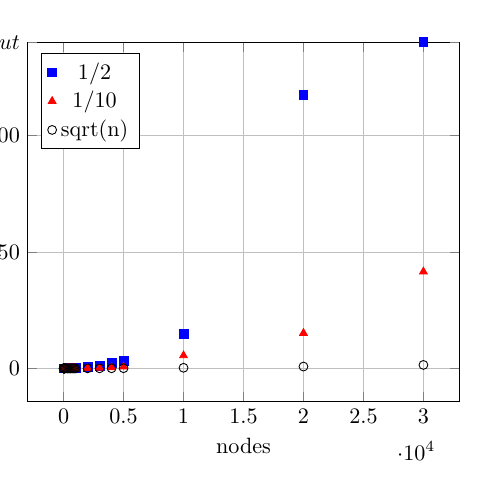
\begin{tikzpicture}[trim left=0cm, scale=0.8]
	\begin{axis}[
		xlabel=nodes,
		ylabel=t sec,
		legend pos=north west,
		grid=both,
		  extra y ticks={140},
		  extra tick style={grid=major, grid style={dotted, cyan}},
		  extra y tick labels={\hspace{5em}$timeout$},
		  extra x tick labels={},
		  extra y tick style={grid=none},
		  ymax=140
	]
	\addplot[
		scatter,only marks,scatter src=explicit symbolic,
		scatter/classes={
		  	a={mark=square*,blue},
		  	b={mark=triangle*,red},
		  	c={mark=o,draw=black,fill=black}
		}
	]
	table[x=x,y=y,meta=label]{
	  	x    y    label
	  	5	0.000801086425781	a
	  	10	0.000857830047607	a
	  	15	0.000815868377686	a
	  	20	0.00086498260498	a
	  	25	0.000833034515381	a
	  	30	0.000885009765625	a
	  	40	0.00108909606934	a
	  	50	0.000993013381958	a
	  	60	0.00110292434692	a
	  	70	0.00121307373047	a
	  	80	0.0013689994812	a
	  	100	0.00164794921875	a
	  	200	0.00490808486938	a
	  	300	0.0093150138855	a
	  	400	0.0167360305786	a
	  	500	0.0253059864044	a
	  	600	0.057608127594	a
	  	700	0.0520691871643	a
	  	800	0.0675909519196	a
	  	900	0.0881798267365	a
	  	1000	0.10640001297	a
	  	2000	0.486861944199	a
	  	3000	1.15394091606	a
	  	4000	2.44690203667	a
	  	5000	3.31565213203	a
	  	10000	14.8829817772	a
	  	20000	117.417869091	a
	  	30000	140 a
	  	5	0.000885009765625	b
	  	10	0.000794172286987	b
	  	15	0.000741004943848	b
	  	20	0.000755786895752	b
	  	25	0.000725984573364	b
	  	30	0.000759124755859	b
	  	40	0.000608921051025	b
	  	50	0.000768899917603	b
	  	60	0.000777959823608	b
	  	70	0.00056004524231	b
	  	80	0.000833034515381	b
	  	100	0.000924110412598	b
	  	200	0.00145792961121	b
	  	300	0.00253701210022	b
	  	400	0.00378179550171	b
	  	500	0.00561785697937	b
	  	600	0.00787591934204	b
	  	700	0.0102968215942	b
	  	800	0.0132210254669	b
	  	900	0.0209939479828	b
	  	1000	0.0328350067139	b
	  	2000	0.092490196228	b
	  	3000	0.217137813568	b
	  	4000	0.437031030655	b
	  	5000	0.702178001404	b
	  	10000	5.52752995491	b
	  	20000	15.1563310623	b
	  	30000	41.5227429867	b
	  	5	0.00109505653381	c
	  	10	0.000798940658569	c
	  	15	0.000815153121948	c
	  	20	0.000773906707764	c
	  	25	0.000853061676025	c
	  	30	0.000845909118652	c
	  	40	0.000874042510986	c
	  	50	0.000829935073853	c
	  	60	0.000848054885864	c
	  	70	0.000916004180908	c
	  	80	0.00099515914917	c
	  	100	0.00124502182007	c
	  	200	0.00164079666138	c
	  	300	0.00241208076477	c
	  	400	0.00246500968933	c
	  	500	0.00314116477966	c
	  	600	0.0039529800415	c
	  	700	0.00449395179749	c
	  	800	0.00527095794678	c
	  	900	0.00981688499451	c
	  	1000	0.00788497924805	c
	  	2000	0.0212609767914	c
	  	3000	0.0376129150391	c
	  	4000	0.0647239685059	c
	  	5000	0.0853998661041	c
	  	10000	0.264319896698	c
	  	20000	0.797810077667	c
	  	30000	1.4938249588	c
	};
	\legend{1/2, 1/10,sqrt(n)}
	\end{axis}
	\end{tikzpicture}
	
	\caption{Extended random graphs up to 30,000 nodes}
\end{figure}

\newpage
\subsubsection{Cai-Furer-Immerman Graphs}
Another notable graph family are the Cai-Furer-Immerman graphs, also known as CFI. These constructions are resistant to the 1-dimensional Weisfeller-Lehman tests and variants, but are prone to being factored by automorphisms in Traces. See Figure \ref{fig:cfi}.

\subsubsection{Other Graphs}
Other notable graphs which we include here are graphs which were amongst the slowest executing. These include Hadamard (had), Disjoint union of triparite graphs (tnn) and projective planes of order 25 (pp). Note that on the $x$ axis of pp graphs we select only the graphs which have 1302 nodes. thus, the $x$ axis only represents the label of the graph.

\begin{figure}[htbp!]
	\centering
	\begin{minipage}{.4\textwidth}
		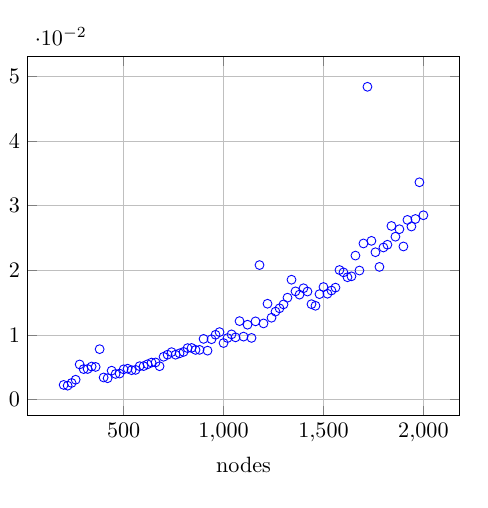
\begin{tikzpicture}[trim left=0cm, scale=0.8]
		\begin{axis}[
		xlabel=nodes,
		ylabel=t sec,
		grid=both
		]
		\addplot[
		scatter,only marks,scatter src=explicit symbolic,
		scatter/classes={
			a={mark=o,blue}
		}
		]
		table[x=x,y=y,meta=label]{
			x    y    label
			200	0.00228190422058	a
			220	0.00216603279114	a
			240	0.0025839805603	a
			260	0.00308394432068	a
			280	0.00544500350952	a
			300	0.00472712516785	a
			320	0.00474214553833	a
			340	0.00512409210205	a
			360	0.0050630569458	a
			380	0.00780987739563	a
			400	0.00343179702759	a
			420	0.00331783294678	a
			440	0.00448203086853	a
			460	0.00397682189941	a
			480	0.0040340423584	a
			500	0.0046911239624	a
			520	0.00479102134705	a
			540	0.0045599937439	a
			560	0.00460505485535	a
			580	0.00517892837524	a
			600	0.00519204139709	a
			620	0.00547194480896	a
			640	0.00573587417603	a
			660	0.0057520866394	a
			680	0.00517296791077	a
			700	0.0066339969635	a
			720	0.00695490837097	a
			740	0.00734996795654	a
			760	0.00695300102234	a
			780	0.00716400146484	a
			800	0.00738596916199	a
			820	0.00797080993652	a
			840	0.00799918174744	a
			860	0.00769591331482	a
			880	0.00770401954651	a
			900	0.00939702987671	a
			920	0.00758194923401	a
			940	0.00934600830078	a
			960	0.0100378990173	a
			980	0.0104479789734	a
			1000	0.00875687599182	a
			1020	0.00953316688538	a
			1040	0.010097026825	a
			1060	0.00963497161865	a
			1080	0.0121469497681	a
			1100	0.00975108146667	a
			1120	0.0115921497345	a
			1140	0.00955009460449	a
			1160	0.0121080875397	a
			1180	0.0208129882812	a
			1200	0.0117888450623	a
			1220	0.0148329734802	a
			1240	0.0126678943634	a
			1260	0.0136151313782	a
			1280	0.0141289234161	a
			1300	0.0147290229797	a
			1320	0.0157740116119	a
			1340	0.0185480117798	a
			1360	0.0167479515076	a
			1380	0.0162441730499	a
			1400	0.0172300338745	a
			1420	0.0167219638824	a
			1440	0.0147659778595	a
			1460	0.0145189762115	a
			1480	0.0163161754608	a
			1500	0.0174181461334	a
			1520	0.0163819789886	a
			1540	0.0168778896332	a
			1560	0.0173258781433	a
			1580	0.0200490951538	a
			1600	0.0196859836578	a
			1620	0.0189318656921	a
			1640	0.019070148468	a
			1660	0.0222799777985	a
			1680	0.0199689865112	a
			1700	0.0241541862488	a
			1720	0.0483820438385	a
			1740	0.0245571136475	a
			1760	0.0227990150452	a
			1780	0.0205280780792	a
			1800	0.0235340595245	a
			1820	0.0239598751068	a
			1840	0.0268609523773	a
			1860	0.0251989364624	a
			1880	0.0263600349426	a
			1900	0.0236899852753	a
			1920	0.0277979373932	a
			1940	0.0267760753632	a
			1960	0.027941942215	a
			1980	0.0336151123047	a
			2000	0.0285170078278	a
		};
		\end{axis}
		\end{tikzpicture}
		
	\end{minipage}
	\begin{minipage}{.4\textwidth}
		\centering
		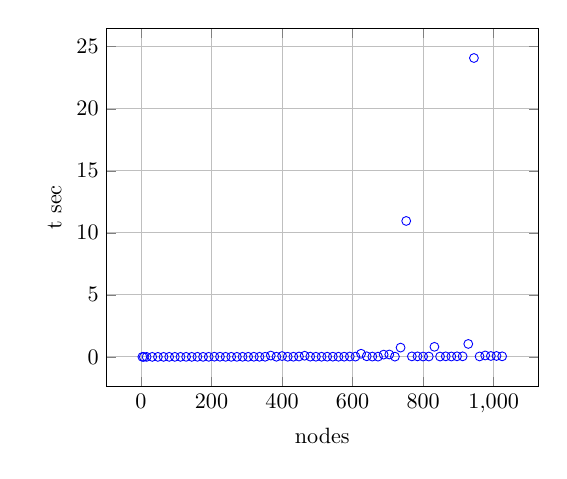
\begin{tikzpicture}[trim left=-1cm, scale=0.8]
		\begin{axis}[
		xlabel=nodes,
		ylabel=t sec,
		grid=both
		]
		\addplot[
		scatter,only marks,scatter src=explicit symbolic,
		scatter/classes={
			a={mark=o,blue}
		}
		]
		table[x=x,y=y,meta=label]{
			x    y    label
			4	0.000930070877075	a
			8	0.000865936279297	a
			16	0.000845193862915	a
			32	0.000930786132812	a
			48	0.00147294998169	a
			64	0.00136494636536	a
			80	0.00255489349365	a
			96	0.00285792350769	a
			112	0.00303387641907	a
			128	0.00530004501343	a
			144	0.00288701057434	a
			160	0.00666308403015	a
			176	0.00345611572266	a
			192	0.00493788719177	a
			208	0.0167338848114	a
			224	0.0145990848541	a
			240	0.00622987747192	a
			256	0.00490307807922	a
			272	0.00505113601685	a
			288	0.00681591033936	a
			304	0.00606393814087	a
			320	0.0118939876556	a
			336	0.0076220035553	a
			352	0.0107100009918	a
			368	0.1057908535	a
			384	0.0120139122009	a
			400	0.0673158168793	a
			416	0.0125169754028	a
			432	0.0138850212097	a
			448	0.0296130180359	a
			464	0.093101978302	a
			480	0.0204088687897	a
			496	0.0136818885803	a
			512	0.0128610134125	a
			528	0.017657995224	a
			544	0.0184848308563	a
			560	0.0129160881042	a
			576	0.0185670852661	a
			592	0.0293200016022	a
			608	0.0233659744263	a
			624	0.253060817719	a
			640	0.0492939949036	a
			656	0.0243890285492	a
			672	0.0193901062012	a
			688	0.183281898499	a
			704	0.194499969482	a
			720	0.0207889080048	a
			736	0.749053001404	a
			752	10.9565410614	a
			768	0.0408179759979	a
			784	0.0409290790558	a
			800	0.029314994812	a
			816	0.0302150249481	a
			832	0.811336994171	a
			848	0.0284330844879	a
			864	0.0446970462799	a
			880	0.0330929756165	a
			896	0.0468261241913	a
			912	0.0451979637146	a
			928	1.04390501976	a
			944	24.0905220509	a
			960	0.0360689163208	a
			976	0.116590023041	a
			992	0.0725729465485	a
			1008	0.0731618404388	a
			1024	0.0454850196838	a
		};
		\end{axis}
		\end{tikzpicture}
	\end{minipage}
	\captionsetup{justification=centering}
	\caption{Left: Cai-Furer-Immerman graphs (cfi).
		Right: Hadamard (had). }
	
	\label{fig:cfi}
\end{figure}
\begin{figure}[htbp!] 
	\centering
	\begin{minipage}{.4\textwidth}
		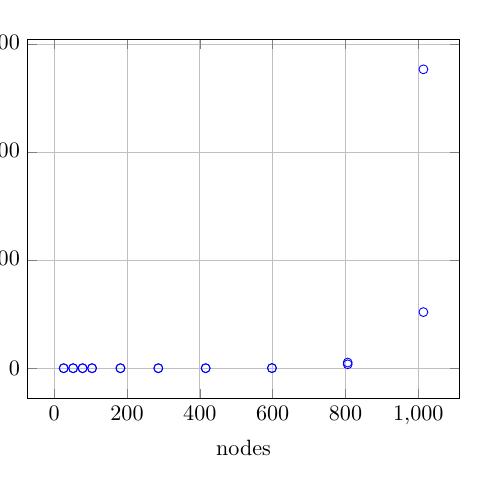
\begin{tikzpicture}[trim left=0cm, scale=0.8]
		\begin{axis}[
		xlabel=nodes,
		ylabel=t sec,
		grid=both
		]
		\addplot[
		scatter,only marks,scatter src=explicit symbolic,
		scatter/classes={
			a={mark=o,blue}
		}
		]
		table[x=x,y=y,meta=label]{
			x    y    label
			26	0.000897169113159	a
			26	0.000981092453003	a
			52	0.0010359287262	a
			52	0.00107097625732	a
			78	0.00181889533997	a
			78	0.00164103507996	a
			104	0.00313401222229	a
			104	0.00259685516357	a
			182	0.0143599510193	a
			182	0.0137579441071	a
			286	0.0655310153961	a
			286	0.0696680545807	a
			416	0.350058078766	a
			416	0.397336959839	a
			598	2.66647791862	a
			598	2.50128698349	a
			806	72.1839659214	a
			806	104.950797796	a
			1014	1039.76025891	a
			1014	5536.82137489	a
		};
		\end{axis}
		\end{tikzpicture}
		
	\end{minipage}
	\begin{minipage}{.4\textwidth}
		\centering
		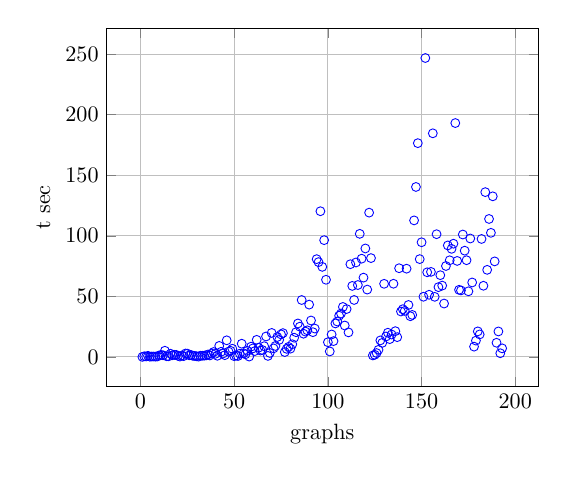
\begin{tikzpicture}[trim left=-1cm, scale=0.8]
		\begin{axis}[
		xlabel=graphs,
		ylabel=t sec,
		grid=both
		]
		\addplot[
		scatter,only marks,scatter src=explicit symbolic,
		scatter/classes={
			a={mark=o,blue}
		}
		]
		table[x=x,y=y,meta=label]{
			x    y    label
			1	0.0126891136169	a
			2	0.506518125534	a
			3	0.392946004868	a
			4	0.894825935364	a
			5	0.196982145309	a
			6	0.315265893936	a
			7	0.332309007645	a
			8	0.24335193634	a
			9	0.365062952042	a
			10	1.23158407211	a
			11	1.57859182358	a
			12	1.39838004112	a
			13	5.08932209015	a
			14	0.509947776794	a
			15	0.502409934998	a
			16	2.62835597992	a
			17	1.43174910545	a
			18	1.66480398178	a
			19	1.67586994171	a
			20	0.863186120987	a
			21	0.319430112839	a
			22	1.08262300491	a
			23	0.651422977448	a
			24	2.7789580822	a
			25	2.71859312057	a
			26	1.33379912376	a
			27	1.57668685913	a
			28	0.861810922623	a
			29	0.814624786377	a
			30	0.491320848465	a
			31	0.250020027161	a
			32	0.979526042938	a
			33	0.990874052048	a
			34	1.03750896454	a
			35	1.27122998238	a
			36	1.9730348587	a
			37	1.21517491341	a
			38	2.7824409008	a
			39	4.03445410728	a
			40	2.57081913948	a
			41	0.918713092804	a
			42	9.09311699867	a
			43	4.21852302551	a
			44	2.79935503006	a
			45	1.44041419029	a
			46	13.6960690022	a
			47	4.36718392372	a
			48	5.09262704849	a
			49	6.74439191818	a
			50	0.615566968918	a
			51	1.09924292564	a
			52	0.72227191925	a
			53	2.66123700142	a
			54	10.8986420631	a
			55	2.99331498146	a
			56	2.17653799057	a
			57	4.99392914772	a
			58	0.269629955292	a
			59	8.45138192177	a
			60	7.03433990479	a
			61	4.83216118813	a
			62	14.0986180305	a
			63	7.55382990837	a
			64	5.27514886856	a
			65	5.73121118546	a
			66	8.84520196915	a
			67	16.8682918549	a
			68	0.821696996689	a
			69	3.25065207481	a
			70	19.8054749966	a
			71	7.05913996696	a
			72	9.04616904259	a
			73	16.4374980927	a
			74	14.0369989872	a
			75	18.596724987	a
			76	19.6481587887	a
			77	4.02276992798	a
			78	6.64521002769	a
			79	8.28684687614	a
			80	6.80820798874	a
			81	10.4670460224	a
			82	15.8501479626	a
			83	20.3741481304	a
			84	27.618694067	a
			85	24.964400053	a
			86	46.9837210178	a
			87	19.1491539478	a
			88	20.89427495	a
			89	21.9608399868	a
			90	43.1752519608	a
			91	30.0575361252	a
			92	20.4183228016	a
			93	23.412883997	a
			94	80.7262451649	a
			95	78.2650489807	a
			96	120.296578169	a
			97	74.3564841747	a
			98	96.4089720249	a
			99	63.7082958221	a
			100	12.1158969402	a
			101	4.52894186974	a
			102	18.5163187981	a
			103	13.0482230186	a
			104	27.6333100796	a
			105	29.2300360203	a
			106	34.0243089199	a
			107	35.8039569855	a
			108	41.2593259811	a
			109	25.9144899845	a
			110	39.5159361362	a
			111	20.2451028824	a
			112	76.5514740944	a
			113	58.6134080887	a
			114	47.0111908913	a
			115	77.9892430305	a
			116	59.3557500839	a
			117	101.617552996	a
			118	81.1093401909	a
			119	65.4591360092	a
			120	89.5387251377	a
			121	55.5878548622	a
			122	119.133154154	a
			123	81.5896930695	a
			124	1.21177482605	a
			125	1.75107908249	a
			126	3.16632509232	a
			127	5.85905790329	a
			128	13.6343200207	a
			129	11.5833981037	a
			130	60.361068964	a
			131	16.8550169468	a
			132	19.9720609188	a
			133	14.6795189381	a
			134	18.4900779724	a
			135	60.4171149731	a
			136	21.2625060081	a
			137	16.3078711033	a
			138	73.2241489887	a
			139	37.4852869511	a
			140	39.396668911	a
			141	37.9996068478	a
			142	72.8519239426	a
			143	42.8854019642	a
			144	33.5778288841	a
			145	34.6762301922	a
			146	112.730048895	a
			147	140.33611393	a
			148	176.509591818	a
			149	80.7491970062	a
			150	94.6595630646	a
			151	49.6790251732	a
			152	246.82178092	a
			153	69.8646960258	a
			154	51.3075819016	a
			155	70.2098720074	a
			156	184.636925936	a
			157	49.6054208279	a
			158	101.324445009	a
			159	57.6079769135	a
			160	67.4897480011	a
			161	58.8694310188	a
			162	44.0615730286	a
			163	75.0678899288	a
			164	92.0624268055	a
			165	79.7877941132	a
			166	89.2363080978	a
			167	93.4773800373	a
			168	193.113031864	a
			169	79.252243042	a
			170	55.3960778713	a
			171	54.9066729546	a
			172	101.057892084	a
			173	87.735656023	a
			174	79.8475270271	a
			175	54.1665978432	a
			176	97.7655980587	a
			177	61.4682059288	a
			178	8.47392106056	a
			179	13.4529950619	a
			180	21.0682308674	a
			181	18.5667409897	a
			182	97.3982541561	a
			183	58.7448019981	a
			184	136.06845212	a
			185	71.8858149052	a
			186	113.916485071	a
			187	102.455598116	a
			188	132.602149963	a
			189	78.8722600937	a
			190	11.6795489788	a
			191	21.0182368755	a
			192	3.02556014061	a
			193	7.06277894974	a
		};
		\end{axis}
		\end{tikzpicture}
	\end{minipage}
	\captionsetup{justification=centering}
	\caption{Left: Disjoint union of tripartite graphs (tnn).\\
		Right: Projective planes of order 25 containing 1302 nodes (pp). }
\end{figure}

\newpage
\section{Results}
Here we present the performance of our construction for varying node sizes. 

\subsection{Packages}
Since we range our systems in complexity and along different rations, we package our graphs into three: $n=m$, $2n=m$ and smallest ratios found. Given that we stop finding systems for a reasonable number of tries at 139 for $n=m$, we continue searching the closest we can, without having to ramp up the try value. Hence, for the most part, tries were left at 10, and we performed and Advanced Search with multiple iterations (>30), updating k-locally consistent systems and checking for automorphisms on the fly. We then executed some logic to separate these packages along the lines defined above. Of course, we could have had more lines, say $3n=m$ and $xn=m$, where $1<x<2$. But our results proved satisfactory to show distinctive times. We did provide more packages, but we will focus on these for now. Figure \ref{fig:inst} best describes what we mean by various lines and instances found for $n$ and $m$. Note that these instances are not necessarily $k$-locally consistent. 


\begin{figure}[h]
	\centering
	  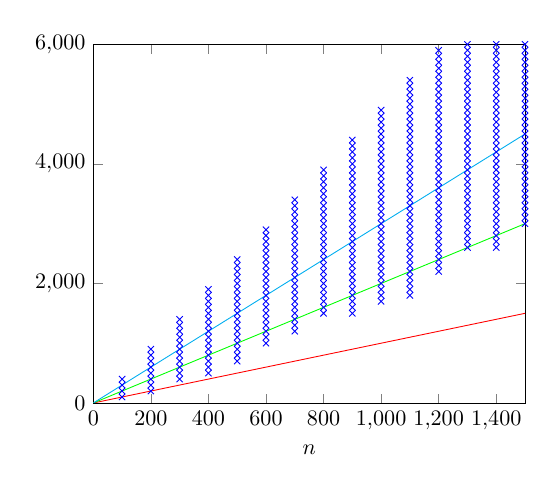
\begin{tikzpicture}[scale=0.8]
		\begin{axis}[
		compat=newest,
		xmin=0,
		xmax=1500,
		ymin=0,
		ymax=6000,
		xlabel={$n$}
		]
		\addplot[
		scatter,only marks,scatter src=explicit symbolic,
		scatter/classes={
			a={mark=x,blue}
		}
		]
		table[x=x,y=y,meta=label]{
			x    y    label
			100  100 a
			100  200 a
			100  300 a
			100  400 a
			200  200 a
			200  300 a
			200  400 a
			200  500 a
			200  600 a
			200  700 a
			200  800 a
			200  900 a
			300  400 a
			300  500 a
			300  600 a
			300  700 a
			300  800 a
			300  900 a
			300  1000 a
			300  1100 a
			300  1200 a
			300  1300 a
			300  1400 a
			400  500 a
			400  600 a
			400  700 a
			400  800 a
			400  900 a
			400  1000 a
			400  1100 a
			400  1200 a
			400  1300 a
			400  1400 a
			400  1500 a
			400  1600 a
			400  1700 a
			400  1800 a
			400  1900 a
			500  700 a
			500  800 a
			500  900 a
			500  1000 a
			500  1100 a
			500  1200 a
			500  1300 a
			500  1400 a
			500  1500 a
			500  1600 a
			500  1700 a
			500  1800 a
			500  1900 a
			500  2000 a
			500  2100 a
			500  2200 a
			500  2300 a
			500  2400 a
			600  1000 a
			600  1100 a
			600  1200 a
			600  1300 a
			600  1400 a
			600  1500 a
			600  1600 a
			600  1700 a
			600  1800 a
			600  1900 a
			600  2000 a
			600  2100 a
			600  2200 a
			600  2300 a
			600  2400 a
			600  2500 a
			600  2600 a
			600  2700 a
			600  2800 a
			600  2900 a
			700  1200 a
			700  1300 a
			700  1400 a
			700  1500 a
			700  1600 a
			700  1700 a
			700  1800 a
			700  1900 a
			700  2000 a
			700  2100 a
			700  2200 a
			700  2300 a
			700  2400 a
			700  2500 a
			700  2600 a
			700  2700 a
			700  2800 a
			700  2900 a
			700  3000 a
			700  3100 a
			700  3200 a
			700  3300 a
			700  3400 a
			800  1500 a
			800  1600 a
			800  1700 a
			800  1800 a
			800  1900 a
			800  2000 a
			800  2100 a
			800  2200 a
			800  2300 a
			800  2400 a
			800  2500 a
			800  2600 a
			800  2700 a
			800  2800 a
			800  2900 a
			800  3000 a
			800  3100 a
			800  3200 a
			800  3300 a
			800  3400 a
			800  3500 a
			800  3600 a
			800  3700 a
			800  3800 a
			800  3900 a
			900  1500 a
			900  1600 a
			900  1700 a
			900  1800 a
			900  1900 a
			900  2000 a
			900  2100 a
			900  2200 a
			900  2300 a
			900  2400 a
			900  2500 a
			900  2600 a
			900  2700 a
			900  2800 a
			900  2900 a
			900  3000 a
			900  3100 a
			900  3200 a
			900  3300 a
			900  3400 a
			900  3500 a
			900  3600 a
			900  3700 a
			900  3800 a
			900  3900 a
			900  4000 a
			900  4100 a
			900  4200 a
			900  4300 a
			900  4400 a
			1000  1700 a
			1000  1800 a
			1000  1900 a
			1000  2000 a
			1000  2100 a
			1000  2200 a
			1000  2300 a
			1000  2400 a
			1000  2500 a
			1000  2600 a
			1000  2700 a
			1000  2800 a
			1000  2900 a
			1000  3000 a
			1000  3100 a
			1000  3200 a
			1000  3300 a
			1000  3400 a
			1000  3500 a
			1000  3600 a
			1000  3700 a
			1000  3800 a
			1000  3900 a
			1000  4000 a
			1000  4100 a
			1000  4200 a
			1000  4300 a
			1000  4400 a
			1000  4500 a
			1000  4600 a
			1000  4700 a
			1000  4800 a
			1000  4900 a
			1100  1800 a
			1100  1900 a
			1100  2000 a
			1100  2100 a
			1100  2200 a
			1100  2300 a
			1100  2400 a
			1100  2500 a
			1100  2600 a
			1100  2700 a
			1100  2800 a
			1100  2900 a
			1100  3000 a
			1100  3100 a
			1100  3200 a
			1100  3300 a
			1100  3400 a
			1100  3500 a
			1100  3600 a
			1100  3700 a
			1100  3800 a
			1100  3900 a
			1100  4000 a
			1100  4100 a
			1100  4200 a
			1100  4300 a
			1100  4400 a
			1100  4500 a
			1100  4600 a
			1100  4700 a
			1100  4800 a
			1100  4900 a
			1100  5000 a
			1100  5100 a
			1100  5200 a
			1100  5300 a
			1100  5400 a
			1200  2200 a
			1200  2300 a
			1200  2400 a
			1200  2500 a
			1200  2600 a
			1200  2700 a
			1200  2800 a
			1200  2900 a
			1200  3000 a
			1200  3100 a
			1200  3200 a
			1200  3300 a
			1200  3400 a
			1200  3500 a
			1200  3600 a
			1200  3700 a
			1200  3800 a
			1200  3900 a
			1200  4000 a
			1200  4100 a
			1200  4200 a
			1200  4300 a
			1200  4400 a
			1200  4500 a
			1200  4600 a
			1200  4700 a
			1200  4800 a
			1200  4900 a
			1200  5000 a
			1200  5100 a
			1200  5200 a
			1200  5300 a
			1200  5400 a
			1200  5500 a
			1200  5600 a
			1200  5700 a
			1200  5800 a
			1200  5900 a
			1300  2600 a
			1300  2700 a
			1300  2800 a
			1300  2900 a
			1300  3000 a
			1300  3100 a
			1300  3200 a
			1300  3300 a
			1300  3400 a
			1300  3500 a
			1300  3600 a
			1300  3700 a
			1300  3800 a
			1300  3900 a
			1300  4000 a
			1300  4100 a
			1300  4200 a
			1300  4300 a
			1300  4400 a
			1300  4500 a
			1300  4600 a
			1300  4700 a
			1300  4800 a
			1300  4900 a
			1300  5000 a
			1300  5100 a
			1300  5200 a
			1300  5300 a
			1300  5400 a
			1300  5500 a
			1300  5600 a
			1300  5700 a
			1300  5800 a
			1300  5900 a
			1300  6000 a
			1300  6100 a
			1300  6200 a
			1300  6300 a
			1300  6400 a
			1400  2600 a
			1400  2700 a
			1400  2800 a
			1400  2900 a
			1400  3000 a
			1400  3100 a
			1400  3200 a
			1400  3300 a
			1400  3400 a
			1400  3500 a
			1400  3600 a
			1400  3700 a
			1400  3800 a
			1400  3900 a
			1400  4000 a
			1400  4100 a
			1400  4200 a
			1400  4300 a
			1400  4400 a
			1400  4500 a
			1400  4600 a
			1400  4700 a
			1400  4800 a
			1400  4900 a
			1400  5000 a
			1400  5100 a
			1400  5200 a
			1400  5300 a
			1400  5400 a
			1400  5500 a
			1400  5600 a
			1400  5700 a
			1400  5800 a
			1400  5900 a
			1400  6000 a
			1400  6100 a
			1400  6200 a
			1400  6300 a
			1400  6400 a
			1400  6500 a
			1400  6600 a
			1400  6700 a
			1400  6800 a
			1400  6900 a
			1500  3000 a
			1500  3100 a
			1500  3200 a
			1500  3300 a
			1500  3400 a
			1500  3500 a
			1500  3600 a
			1500  3700 a
			1500  3800 a
			1500  3900 a
			1500  4000 a
			1500  4100 a
			1500  4200 a
			1500  4300 a
			1500  4400 a
			1500  4500 a
			1500  4600 a
			1500  4700 a
			1500  4800 a
			1500  4900 a
			1500  5000 a
			1500  5100 a
			1500  5200 a
			1500  5300 a
			1500  5400 a
			1500  5500 a
			1500  5600 a
			1500  5700 a
			1500  5800 a
			1500  5900 a
			1500  6000 a
			1500  6100 a
			1500  6200 a
			1500  6300 a
			1500  6400 a
			1500  6500 a
			1500  6600 a
			1500  6700 a
			1500  6800 a
			1500  6900 a
			1500  7000 a
			1500  7100 a
			1500  7200 a
			1500  7300 a
			1500  7400 a
			1600  3200 a
			1600  3300 a
			1600  3400 a
			1600  3500 a
			1600  3600 a
			1600  3700 a
			1600  3800 a
			1600  3900 a
			1600  4000 a
			1600  4100 a
			1600  4200 a
			1600  4300 a
			1600  4400 a
			1600  4500 a
			1600  4600 a
			1600  4700 a
			1600  4800 a
			1600  4900 a
			1600  5000 a
			1600  5100 a
			1600  5200 a
			1600  5300 a
			1600  5400 a
			1600  5500 a
			1600  5600 a
			1600  5700 a
			1600  5800 a
			1600  5900 a
			1600  6000 a
			1600  6100 a
			1600  6200 a
			1600  6300 a
			1600  6400 a
			1600  6500 a
			1600  6600 a
			1600  6700 a
			1600  6800 a
			1600  6900 a
			1600  7000 a
			1600  7100 a
			1600  7200 a
			1600  7300 a
			1600  7400 a
			1600  7500 a
			1600  7600 a
			1600  7700 a
			1600  7800 a
			1600  7900 a
			1700  3300 a
			1700  3400 a
			1700  3500 a
			1700  3600 a
			1700  3700 a
			1700  3800 a
			1700  3900 a
			1700  4000 a
			1700  4100 a
			1700  4200 a
			1700  4300 a
			1700  4400 a
			1700  4500 a
			1700  4600 a
			1700  4700 a
			1700  4800 a
			1700  4900 a
			1700  5000 a
			1700  5100 a
			1700  5200 a
			1700  5300 a
			1700  5400 a
			1700  5500 a
			1700  5600 a
			1700  5700 a
			1700  5800 a
			1700  5900 a
			1700  6000 a
			1700  6100 a
			1700  6200 a
			1700  6300 a
			1700  6400 a
			1700  6500 a
			1700  6600 a
			1700  6700 a
			1700  6800 a
			1700  6900 a
			1700  7000 a
			1700  7100 a
			1700  7200 a
			1700  7300 a
			1700  7400 a
			1700  7500 a
			1700  7600 a
			1700  7700 a
			1700  7800 a
			1700  7900 a
			1700  8000 a
			1700  8100 a
			1700  8200 a
			1700  8300 a
			1700  8400 a
			1800  3900 a
			1800  4000 a
			1800  4100 a
			1800  4200 a
			1800  4300 a
			1800  4400 a
			1800  4500 a
			1800  4600 a
			1800  4700 a
			1800  4800 a
			1800  4900 a
			1800  5000 a
			1800  5100 a
			1800  5200 a
			1800  5300 a
			1800  5400 a
			1800  5500 a
			1800  5600 a
			1800  5700 a
			1800  5800 a
			1800  5900 a
			1800  6000 a
			1800  6100 a
			1800  6200 a
			1800  6300 a
			1800  6400 a
			1800  6500 a
			1800  6600 a
			1800  6700 a
			1800  6800 a
			1800  6900 a
			1800  7000 a
			1800  7100 a
			1800  7200 a
			1800  7300 a
			1800  7400 a
			1800  7500 a
			1800  7600 a
			1800  7700 a
			1800  7800 a
			1800  7900 a
			1800  8000 a
			1800  8100 a
			1800  8200 a
			1800  8300 a
			1800  8400 a
			1800  8500 a
			1800  8600 a
			1800  8700 a
			1800  8800 a
			1800  8900 a
			1900  4000 a
			1900  4100 a
			1900  4200 a
			1900  4300 a
			1900  4400 a
			1900  4500 a
			1900  4600 a
			1900  4700 a
			1900  4800 a
			1900  4900 a
			1900  5000 a
			1900  5100 a
			1900  5200 a
			1900  5300 a
			1900  5400 a
			1900  5500 a
			1900  5600 a
			1900  5700 a
			1900  5800 a
			1900  5900 a
			1900  6000 a
			1900  6100 a
			1900  6200 a
			1900  6300 a
			1900  6400 a
			1900  6500 a
			1900  6600 a
			1900  6700 a
			1900  6800 a
			1900  6900 a
			1900  7000 a
			1900  7100 a
			1900  7200 a
			1900  7300 a
			1900  7400 a
			1900  7500 a
			1900  7600 a
			1900  7700 a
			1900  7800 a
			1900  7900 a
			1900  8000 a
			1900  8100 a
			1900  8200 a
			1900  8300 a
			1900  8400 a
			1900  8500 a
			1900  8600 a
			1900  8700 a
			1900  8800 a
			1900  8900 a
			1900  9000 a
			1900  9100 a
			1900  9200 a
			1900  9300 a
			1900  9400 a
			2000  2000 a
			2000  2100 a
			2000  2200 a
			2000  2300 a
			2000  2400 a
			2000  2500 a
			2000  2600 a
			2000  2700 a
			2000  2800 a
			2000  2900 a
			2000  3000 a
			2000  3100 a
			2000  3200 a
			2000  3300 a
			2000  3400 a
			2000  3500 a
			2000  3600 a
			2000  3700 a
			2000  3800 a
			2000  3900 a
			2000  4000 a
			2000  4100 a
			2000  4200 a
			2000  4300 a
			2000  4400 a
			2000  4500 a
			2000  4600 a
			2000  4700 a
			2000  4800 a
			2000  4900 a
			2000  5000 a
			2000  5100 a
			2000  5200 a
			2000  5300 a
			2000  5400 a
			2000  5500 a
			2000  5600 a
			2000  5700 a
			2000  5800 a
			2000  5900 a
			2000  6000 a
			2000  6100 a
			2000  6200 a
			2000  6300 a
			2000  6400 a
			2000  6500 a
			2000  6600 a
			2000  6700 a
			2000  6800 a
			2000  6900 a
			2000  7000 a
			2000  7100 a
			2000  7200 a
			2000  7300 a
			2000  7400 a
			2000  7500 a
			2000  7600 a
			2000  7700 a
			2000  7800 a
			2000  7900 a
			2000  8000 a
			2000  8100 a
			2000  8200 a
			2000  8300 a
			2000  8400 a
			2000  8500 a
			2000  8600 a
			2000  8700 a
			2000  8800 a
			2000  8900 a
			2000  9000 a
			2000  9100 a
			2000  9200 a
			2000  9300 a
			2000  9400 a
			2000  9500 a
			2000  9600 a
			2000  9700 a
			2000  9800 a
			2000  9900 a
			2100  4100 a
			2100  4200 a
			2100  4300 a
			2100  4400 a
			2100  4500 a
			2100  4600 a
			2100  4700 a
			2100  4800 a
			2100  4900 a
			2100  5000 a
			2100  5100 a
			2100  5200 a
			2100  5300 a
			2100  5400 a
			2100  5500 a
			2100  5600 a
			2100  5700 a
			2100  5800 a
			2100  5900 a
			2100  6000 a
			2100  6100 a
			2100  6200 a
			2100  6300 a
			2100  6400 a
			2100  6500 a
			2100  6600 a
			2100  6700 a
			2100  6800 a
			2100  6900 a
			2100  7000 a
			2100  7100 a
			2100  7200 a
			2100  7300 a
			2100  7400 a
			2100  7500 a
			2100  7600 a
			2100  7700 a
			2100  7800 a
			2100  7900 a
			2100  8000 a
			2100  8100 a
			2100  8200 a
			2100  8300 a
			2100  8400 a
			2100  8500 a
			2100  8600 a
			2100  8700 a
			2100  8800 a
			2100  8900 a
			2100  9000 a
			2100  9100 a
			2100  9200 a
			2100  9300 a
			2100  9400 a
			2100  9500 a
			2100  9600 a
			2100  9700 a
			2100  9800 a
			2100  9900 a
			2100  10000 a
			2200  4500 a
			2200  4600 a
			2200  4700 a
			2200  4800 a
			2200  4900 a
			2200  5000 a
			2200  5100 a
			2200  5200 a
			2200  5300 a
			2200  5400 a
			2200  5500 a
			2200  5600 a
			2200  5700 a
			2200  5800 a
			2200  5900 a
			2200  6000 a
			2200  6100 a
			2200  6200 a
			2200  6300 a
			2200  6400 a
			2200  6500 a
			2200  6600 a
			2200  6700 a
			2200  6800 a
			2200  6900 a
			2200  7000 a
			2200  7100 a
			2200  7200 a
			2200  7300 a
			2200  7400 a
			2200  7500 a
			2200  7600 a
			2200  7700 a
			2200  7800 a
			2200  7900 a
			2200  8000 a
			2200  8100 a
			2200  8200 a
			2200  8300 a
			2200  8400 a
			2200  8500 a
			2200  8600 a
			2200  8700 a
			2200  8800 a
			2200  8900 a
			2200  9000 a
			2200  9100 a
			2200  9200 a
			2200  9300 a
			2200  9400 a
			2200  9500 a
			2200  9600 a
			2200  9700 a
			2200  9800 a
			2200  9900 a
			2200  10000 a
			2300  4900 a
			2300  5000 a
			2300  5100 a
			2300  5200 a
			2300  5300 a
			2300  5400 a
			2300  5500 a
			2300  5600 a
			2300  5700 a
			2300  5800 a
			2300  5900 a
			2300  6000 a
			2300  6100 a
			2300  6200 a
			2300  6300 a
			2300  6400 a
			2300  6500 a
			2300  6600 a
			2300  6700 a
			2300  6800 a
			2300  6900 a
			2300  7000 a
			2300  7100 a
			2300  7200 a
			2300  7300 a
			2300  7400 a
			2300  7500 a
			2300  7600 a
			2300  7700 a
			2300  7800 a
			2300  7900 a
			2300  8000 a
			2300  8100 a
			2300  8200 a
			2300  8300 a
			2300  8400 a
			2300  8500 a
			2300  8600 a
			2300  8700 a
			2300  8800 a
			2300  8900 a
			2300  9000 a
			2300  9100 a
			2300  9200 a
			2300  9300 a
			2300  9400 a
			2300  9500 a
			2300  9600 a
			2300  9700 a
			2300  9800 a
			2300  9900 a
			2300  10000 a
			2400  5200 a
			2400  5300 a
			2400  5400 a
			2400  5500 a
			2400  5600 a
			2400  5700 a
			2400  5800 a
			2400  5900 a
			2400  6000 a
			2400  6100 a
			2400  6200 a
			2400  6300 a
			2400  6400 a
			2400  6500 a
			2400  6600 a
			2400  6700 a
			2400  6800 a
			2400  6900 a
			2400  7000 a
			2400  7100 a
			2400  7200 a
			2400  7300 a
			2400  7400 a
			2400  7500 a
			2400  7600 a
			2400  7700 a
			2400  7800 a
			2400  7900 a
			2400  8000 a
			2400  8100 a
			2400  8200 a
			2400  8300 a
			2400  8400 a
			2400  8500 a
			2400  8600 a
			2400  8700 a
			2400  8800 a
			2400  8900 a
			2400  9000 a
			2400  9100 a
			2400  9200 a
			2400  9300 a
			2400  9400 a
			2400  9500 a
			2400  9600 a
			2400  9700 a
			2400  9800 a
			2400  9900 a
			2400  10000 a
		};
		\draw[color=red] (0,0) -- (1500,1500) node[right] {a};
		\draw[color=green] (0,0) -- (1500,3000);
		\draw[color=cyan] (0,0) -- (1500,4500);
		\end{axis}
	  \end{tikzpicture}
	  \caption{Uniquely satisfiable instances found.}{Red: $n=m$; Green: $2n=m$; Cyan:$3n=m$; Crosses: Uniquely satisfiable instances found}
	  \label{fig:inst}
	  
\end{figure}
\newpage
\subsection{Performance}
Here we present the performance of varying packages. Figure \ref{fig:px} displays the timings of the three packages created. Figure \ref{fig:py} illustrates our most difficult package \emph{con\_sml} versus existing benchmarks. Results showed that we consistently produced graphs which executed for longer than three hours, however, since many of the packages did not execute for longer than the specified timeout, we could not compare graphs of equal sizes for most graphs which timed out. 


\begin{figure}[htbp!] 
	\centering
	\begin{minipage}{.4\textwidth}
		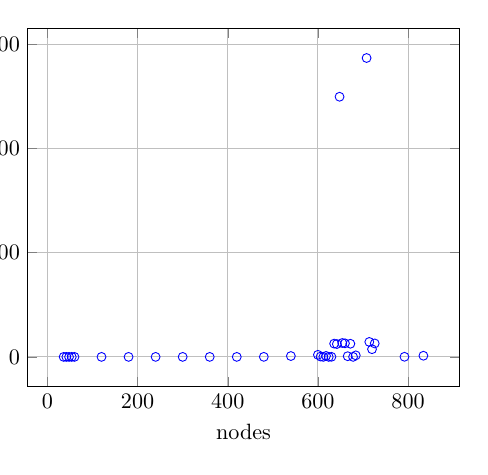
\begin{tikzpicture}[trim left=0cm, scale=0.8]
		\begin{axis}[
		xlabel=nodes,
		ylabel=t sec,
		grid=both,
		]
		\addplot[
		scatter,only marks,scatter src=explicit symbolic,
		scatter/classes={
			a={mark=o,blue}
		}
		]
		table[x=x,y=y,meta=label]{
			x    y    label
			36	0.000504970550537	a
			42	0.000595092773438	a
			48	0.000430107116699	a
			54	0.000416994094849	a
			60	0.000868082046509	a
			120	0.0010769367218	a
			180	0.00196194648743	a
			240	0.0024151802063	a
			300	0.00288486480713	a
			360	0.00310897827148	a
			420	0.00304412841797	a
			480	0.0377099514008	a
			540	0.822341918945	a
			600	1.99121904373	a
			606	0.287495136261	a
			612	0.0140619277954	a
			618	0.919209003448	a
			624	0.014004945755	a
			630	0.0803589820862	a
			636	12.7223041058	a
			642	12.3259220123	a
			648	249.624564171	a
			654	13.3357129097	a
			660	13.0116429329	a
			666	0.671919822693	a
			672	12.6001150608	a
			678	0.0159549713135	a
			684	1.46877002716	a
			708	286.804507017	a
			714	14.3620049953	a
			720	7.38974690437	a
			726	12.9122009277	a
			792	0.103566884995	a
			834	1.10935306549	a
		};
		\end{axis}
		\end{tikzpicture}
		
	\end{minipage}
	\begin{minipage}{.4\textwidth}
		\centering
		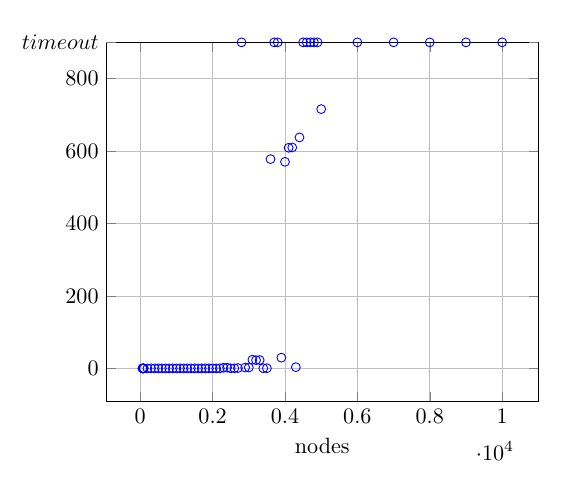
\begin{tikzpicture}[trim left=-1cm, scale=0.8]
		\begin{axis}[
		xlabel=nodes,
		ylabel=t sec,
		grid=both,
		extra y ticks={900},
		extra y tick labels={\hspace{5em}$timeout$},
		extra y tick style={grid=none},
		ymax=900,
		]
		\addplot[
		scatter,only marks,scatter src=explicit symbolic,
		scatter/classes={
			a={mark=o,blue}
		}
		]
		table[x=x,y=y,meta=label]{
			x    y    label
			60	0.00088095664978	a
			70	0.000917196273804	a
			80	0.000850915908813	a
			90	0.000887870788574	a
			100	0.000802040100098	a
			200	0.000893115997314	a
			300	0.00113701820374	a
			400	0.00194406509399	a
			500	0.00256896018982	a
			600	0.00155901908875	a
			700	0.00173497200012	a
			800	0.00396299362183	a
			900	0.00400900840759	a
			1000	0.00220799446106	a
			1100	0.0236101150513	a
			1200	0.00546789169312	a
			1300	0.00626587867737	a
			1400	0.00990104675293	a
			1500	0.0394530296326	a
			1600	0.0112538337708	a
			1700	0.0123739242554	a
			1800	0.0139899253845	a
			1900	0.0278260707855	a
			2000	0.0534319877625	a
			2100	0.00984311103821	a
			2200	0.0178880691528	a
			2300	1.90173387527	a
			2400	2.04471302032	a
			2500	0.200901985168	a
			2600	0.327310085297	a
			2700	0.923086881638	a
			2800	900	a
			2900	2.30818605423	a
			3000	2.48632717133	a
			3100	23.9029829502	a
			3200	22.727894783	a
			3300	23.0080840588	a
			3400	0.441438913345	a
			3500	0.49547791481	a
			3600	577.676494122	a
			3700	900	a
			3800	900	a
			3900	29.6461250782	a
			4000	570.171611071	a
			4100	609.037957907	a
			4200	609.872159004	a
			4300	3.48693990707	a
			4400	637.644945145	a
			4500	900	a
			4600	900	a
			4700	900	a
			4800	900	a
			4900	900	a
			5000	715.732777119	a
			6000	900	a
			7000	900	a
			8000	900	a
			9000	900	a
			10000	900	a
		};
		\end{axis}
		\end{tikzpicture}
	\end{minipage}
	\\	
	\begin{minipage}{.4\textwidth}	
		\centering
		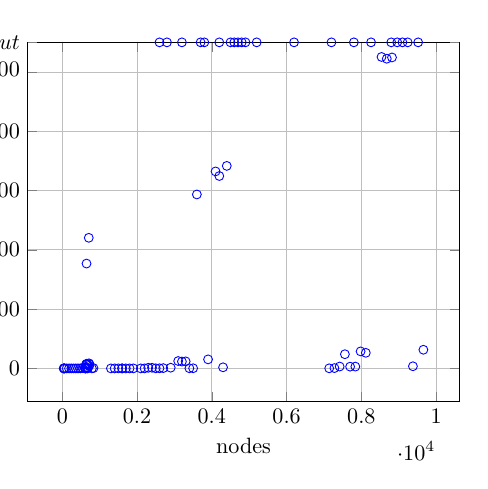
\begin{tikzpicture}[trim left=0cm, scale=0.8]
		\begin{axis}[
		xlabel=nodes,
		ylabel=t sec,
		grid=both,
		extra y ticks={1100},
		extra tick style={grid=major, grid style={dotted, cyan}},
		extra y tick labels={\hspace{5em}$timeout$},
		extra x tick labels={},
		extra y tick style={grid=none},
		ymax=1100
		]
		\addplot[
		scatter,only marks,scatter src=explicit symbolic,
		scatter/classes={
			a={mark=o,blue}
		}
		]
		table[x=x,y=y,meta=label]{
			x    y    label
			36	0.00103306770325	a
			42	0.000981092453003	a
			48	0.000943899154663	a
			54	0.000932931900024	a
			60	0.000885009765625	a
			120	0.00100302696228	a
			180	0.00216317176819	a
			240	0.0023980140686	a
			300	0.00391316413879	a
			360	0.00308299064636	a
			420	0.00360012054443	a
			480	0.0388169288635	a
			540	0.885004997253	a
			600	2.20803809166	a
			606	0.286993980408	a
			612	0.0141770839691	a
			618	1.02969312668	a
			624	0.0157458782196	a
			630	0.0813388824463	a
			636	13.5863618851	a
			642	13.4802289009	a
			648	353.685708046	a
			654	15.9124789238	a
			660	0.967444896698	a
			666	0.688606977463	a
			672	14.1916108131	a
			678	0.0158090591431	a
			684	1.52013897896	a
			708	440.586826086	a
			714	17.1741900444	a
			720	8.75624012947	a
			726	14.2599079609	a
			1300	0.00624203681946	a
			792	0.0990188121796	a
			834	1.13995695114	a
			1400	0.0105519294739	a
			1500	0.0400409698486	a
			1600	0.0119650363922	a
			1700	0.0137841701508	a
			1800	0.0135757923126	a
			1900	0.0268559455872	a
			1600	0.189525842667	a
			2100	0.0101490020752	a
			2200	0.0251288414001	a
			2300	2.07047104836	a
			2400	2.17357993126	a
			2500	0.224191904068	a
			2600	0.327886104584	a
			2700	0.934176206589	a
			2800	1100	a
			2900	2.35056710243	a
			2600	1100	a
			3100	24.9071788788	a
			3200	23.0961768627	a
			3300	23.7306361198	a
			3400	0.444133996964	a
			3500	0.506667852402	a
			3600	586.845415115	a
			3700	1100	a
			3800	1100	a
			3900	30.4615390301	a
			3200	1100	a
			4100	664.525188208	a
			4200	649.032501936	a
			4300	3.69031596184	a
			4400	683.195003986	a
			4500	1100	a
			4600	1100	a
			4700	1100	a
			4800	1100	a
			4900	1100	a
			4200	1100	a
			7140	0.266206026077	a
			7280	1.01169610023	a
			7420	6.30038094521	a
			7560	47.8593740463	a
			7700	5.88605880737	a
			7840	6.14195013046	a
			7980	57.4095039368	a
			8120	52.5715360641	a
			8260	1100	a
			5200	1100	a
			8540	1050.74244285	a
			8680	1044.69068694	a
			8820	1049.08241892	a
			8960	1100	a
			9100	1100	a
			9240	1100	a
			9380	7.24794602394	a
			9520	1100	a
			9660	62.879360199	a
			6200	1100	a
			7200	1100	a
			7800	1100	a
			8800	1100	a
		};
		\end{axis}
		\end{tikzpicture}
	\end{minipage}
	\captionsetup{justification=centering}
	\caption{Left: n=m (con\_n).\\
		Right: n=2m (con\_2n). \\
		Center: smallest ratios found (con\_sml)}
	\label{fig:px}
\end{figure}
\begin{figure}[htbp!]
	\centering
	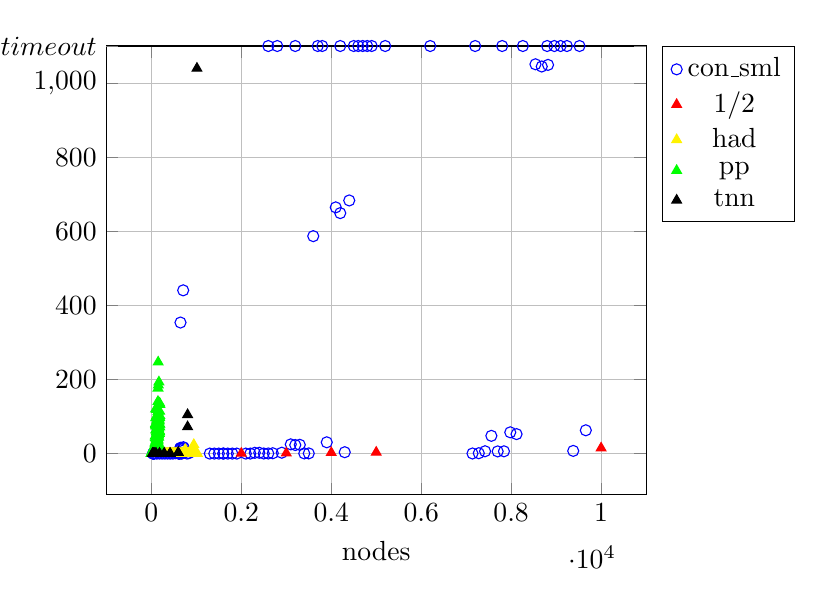
\begin{tikzpicture}[trim left = -1cm, scale=1]
	\begin{axis}[
	xlabel=nodes,
	ylabel=t sec,
	grid=both,
	extra y ticks={1100},
	extra tick style={grid=major, grid style={dotted, cyan}},
	extra y tick labels={\hspace{5em}$timeout$},
	extra x tick labels={},
	extra y tick style={grid=none},
	legend pos=outer north east,
	ymax=1100
	]
	\legend{con\_sml, 1/2, had, pp, tnn}
	\addplot[
	scatter,only marks,scatter src=explicit symbolic,
	scatter/classes={
		a={mark=o,blue},
		b={mark=triangle*,red},
		c={mark=triangle*,yellow},
		d={mark=triangle*,green},
		e={mark=triangle*,black}
	}
	]
	table[x=x,y=y,meta=label]{
		x    y    label
		36	0.00103306770325	a
		42	0.000981092453003	a
		48	0.000943899154663	a
		54	0.000932931900024	a
		60	0.000885009765625	a
		120	0.00100302696228	a
		180	0.00216317176819	a
		240	0.0023980140686	a
		300	0.00391316413879	a
		360	0.00308299064636	a
		420	0.00360012054443	a
		480	0.0388169288635	a
		540	0.885004997253	a
		600	2.20803809166	a
		606	0.286993980408	a
		612	0.0141770839691	a
		618	1.02969312668	a
		624	0.0157458782196	a
		630	0.0813388824463	a
		636	13.5863618851	a
		642	13.4802289009	a
		648	353.685708046	a
		654	15.9124789238	a
		660	0.967444896698	a
		666	0.688606977463	a
		672	14.1916108131	a
		678	0.0158090591431	a
		684	1.52013897896	a
		708	440.586826086	a
		714	17.1741900444	a
		720	8.75624012947	a
		726	14.2599079609	a
		1300	0.00624203681946	a
		792	0.0990188121796	a
		834	1.13995695114	a
		1400	0.0105519294739	a
		1500	0.0400409698486	a
		1600	0.0119650363922	a
		1700	0.0137841701508	a
		1800	0.0135757923126	a
		1900	0.0268559455872	a
		1600	0.189525842667	a
		2100	0.0101490020752	a
		2200	0.0251288414001	a
		2300	2.07047104836	a
		2400	2.17357993126	a
		2500	0.224191904068	a
		2600	0.327886104584	a
		2700	0.934176206589	a
		2800	1100	a
		2900	2.35056710243	a
		2600	1100	a
		3100	24.9071788788	a
		3200	23.0961768627	a
		3300	23.7306361198	a
		3400	0.444133996964	a
		3500	0.506667852402	a
		3600	586.845415115	a
		3700	1100	a
		3800	1100	a
		3900	30.4615390301	a
		3200	1100	a
		4100	664.525188208	a
		4200	649.032501936	a
		4300	3.69031596184	a
		4400	683.195003986	a
		4500	1100	a
		4600	1100	a
		4700	1100	a
		4800	1100	a
		4900	1100	a
		4200	1100	a
		7140	0.266206026077	a
		7280	1.01169610023	a
		7420	6.30038094521	a
		7560	47.8593740463	a
		7700	5.88605880737	a
		7840	6.14195013046	a
		7980	57.4095039368	a
		8120	52.5715360641	a
		8260	1100	a
		5200	1100	a
		8540	1050.74244285	a
		8680	1044.69068694	a
		8820	1049.08241892	a
		8960	1100	a
		9100	1100	a
		9240	1100	a
		9380	7.24794602394	a
		9520	1100	a
		9660	62.879360199	a
		6200	1100	a
		7200	1100	a
		7800	1100	a
		8800	1100	a
		5	0.000801086425781	b
		10	0.000857830047607	b
		15	0.000815868377686	b
		20	0.00086498260498	b
		25	0.000833034515381	b
		30	0.000885009765625	b
		40	0.00108909606934	b
		50	0.000993013381958	b
		60	0.00110292434692	b
		70	0.00121307373047	b
		80	0.0013689994812	b
		100	0.00164794921875	b
		200	0.00490808486938	b
		300	0.0093150138855	b
		400	0.0167360305786	b
		500	0.0253059864044	b
		600	0.057608127594	b
		700	0.0520691871643	b
		800	0.0675909519196	b
		900	0.0881798267365	b
		1000	0.10640001297	b
		2000	0.486861944199	b
		3000	1.15394091606	b
		4000	2.44690203667	b
		5000	3.31565213203	b
		10000	14.8829817772	b
		4	0.000930070877075	c
		8	0.000865936279297	c
		16	0.000845193862915	c
		32	0.000930786132812	c
		48	0.00147294998169	c
		64	0.00136494636536	c
		80	0.00255489349365	c
		96	0.00285792350769	c
		112	0.00303387641907	c
		128	0.00530004501343	c
		144	0.00288701057434	c
		160	0.00666308403015	c
		176	0.00345611572266	c
		192	0.00493788719177	c
		208	0.0167338848114	c
		224	0.0145990848541	c
		240	0.00622987747192	c
		256	0.00490307807922	c
		272	0.00505113601685	c
		288	0.00681591033936	c
		304	0.00606393814087	c
		320	0.0118939876556	c
		336	0.0076220035553	c
		352	0.0107100009918	c
		368	0.1057908535	c
		384	0.0120139122009	c
		400	0.0673158168793	c
		416	0.0125169754028	c
		432	0.0138850212097	c
		448	0.0296130180359	c
		464	0.093101978302	c
		480	0.0204088687897	c
		496	0.0136818885803	c
		512	0.0128610134125	c
		528	0.017657995224	c
		544	0.0184848308563	c
		560	0.0129160881042	c
		576	0.0185670852661	c
		592	0.0293200016022	c
		608	0.0233659744263	c
		624	0.253060817719	c
		640	0.0492939949036	c
		656	0.0243890285492	c
		672	0.0193901062012	c
		688	0.183281898499	c
		704	0.194499969482	c
		720	0.0207889080048	c
		736	0.749053001404	c
		752	10.9565410614	c
		768	0.0408179759979	c
		784	0.0409290790558	c
		800	0.029314994812	c
		816	0.0302150249481	c
		832	0.811336994171	c
		848	0.0284330844879	c
		864	0.0446970462799	c
		880	0.0330929756165	c
		896	0.0468261241913	c
		912	0.0451979637146	c
		928	1.04390501976	c
		944	24.0905220509	c
		960	0.0360689163208	c
		976	0.116590023041	c
		992	0.0725729465485	c
		1008	0.0731618404388	c
		1024	0.0454850196838	c
		1	0.0126891136169	d
		2	0.506518125534	d
		3	0.392946004868	d
		4	0.894825935364	d
		5	0.196982145309	d
		6	0.315265893936	d
		7	0.332309007645	d
		8	0.24335193634	d
		9	0.365062952042	d
		10	1.23158407211	d
		11	1.57859182358	d
		12	1.39838004112	d
		13	5.08932209015	d
		14	0.509947776794	d
		15	0.502409934998	d
		16	2.62835597992	d
		17	1.43174910545	d
		18	1.66480398178	d
		19	1.67586994171	d
		20	0.863186120987	d
		21	0.319430112839	d
		22	1.08262300491	d
		23	0.651422977448	d
		24	2.7789580822	d
		25	2.71859312057	d
		26	1.33379912376	d
		27	1.57668685913	d
		28	0.861810922623	d
		29	0.814624786377	d
		30	0.491320848465	d
		31	0.250020027161	d
		32	0.979526042938	d
		33	0.990874052048	d
		34	1.03750896454	d
		35	1.27122998238	d
		36	1.9730348587	d
		37	1.21517491341	d
		38	2.7824409008	d
		39	4.03445410728	d
		40	2.57081913948	d
		41	0.918713092804	d
		42	9.09311699867	d
		43	4.21852302551	d
		44	2.79935503006	d
		45	1.44041419029	d
		46	13.6960690022	d
		47	4.36718392372	d
		48	5.09262704849	d
		49	6.74439191818	d
		50	0.615566968918	d
		51	1.09924292564	d
		52	0.72227191925	d
		53	2.66123700142	d
		54	10.8986420631	d
		55	2.99331498146	d
		56	2.17653799057	d
		57	4.99392914772	d
		58	0.269629955292	d
		59	8.45138192177	d
		60	7.03433990479	d
		61	4.83216118813	d
		62	14.0986180305	d
		63	7.55382990837	d
		64	5.27514886856	d
		65	5.73121118546	d
		66	8.84520196915	d
		67	16.8682918549	d
		68	0.821696996689	d
		69	3.25065207481	d
		70	19.8054749966	d
		71	7.05913996696	d
		72	9.04616904259	d
		73	16.4374980927	d
		74	14.0369989872	d
		75	18.596724987	d
		76	19.6481587887	d
		77	4.02276992798	d
		78	6.64521002769	d
		79	8.28684687614	d
		80	6.80820798874	d
		81	10.4670460224	d
		82	15.8501479626	d
		83	20.3741481304	d
		84	27.618694067	d
		85	24.964400053	d
		86	46.9837210178	d
		87	19.1491539478	d
		88	20.89427495	d
		89	21.9608399868	d
		90	43.1752519608	d
		91	30.0575361252	d
		92	20.4183228016	d
		93	23.412883997	d
		94	80.7262451649	d
		95	78.2650489807	d
		96	120.296578169	d
		97	74.3564841747	d
		98	96.4089720249	d
		99	63.7082958221	d
		100	12.1158969402	d
		101	4.52894186974	d
		102	18.5163187981	d
		103	13.0482230186	d
		104	27.6333100796	d
		105	29.2300360203	d
		106	34.0243089199	d
		107	35.8039569855	d
		108	41.2593259811	d
		109	25.9144899845	d
		110	39.5159361362	d
		111	20.2451028824	d
		112	76.5514740944	d
		113	58.6134080887	d
		114	47.0111908913	d
		115	77.9892430305	d
		116	59.3557500839	d
		117	101.617552996	d
		118	81.1093401909	d
		119	65.4591360092	d
		120	89.5387251377	d
		121	55.5878548622	d
		122	119.133154154	d
		123	81.5896930695	d
		124	1.21177482605	d
		125	1.75107908249	d
		126	3.16632509232	d
		127	5.85905790329	d
		128	13.6343200207	d
		129	11.5833981037	d
		130	60.361068964	d
		131	16.8550169468	d
		132	19.9720609188	d
		133	14.6795189381	d
		134	18.4900779724	d
		135	60.4171149731	d
		136	21.2625060081	d
		137	16.3078711033	d
		138	73.2241489887	d
		139	37.4852869511	d
		140	39.396668911	d
		141	37.9996068478	d
		142	72.8519239426	d
		143	42.8854019642	d
		144	33.5778288841	d
		145	34.6762301922	d
		146	112.730048895	d
		147	140.33611393	d
		148	176.509591818	d
		149	80.7491970062	d
		150	94.6595630646	d
		151	49.6790251732	d
		152	246.82178092	d
		153	69.8646960258	d
		154	51.3075819016	d
		155	70.2098720074	d
		156	184.636925936	d
		157	49.6054208279	d
		158	101.324445009	d
		159	57.6079769135	d
		160	67.4897480011	d
		161	58.8694310188	d
		162	44.0615730286	d
		163	75.0678899288	d
		164	92.0624268055	d
		165	79.7877941132	d
		166	89.2363080978	d
		167	93.4773800373	d
		168	193.113031864	d
		169	79.252243042	d
		170	55.3960778713	d
		171	54.9066729546	d
		172	101.057892084	d
		173	87.735656023	d
		174	79.8475270271	d
		175	54.1665978432	d
		176	97.7655980587	d
		177	61.4682059288	d
		178	8.47392106056	d
		179	13.4529950619	d
		180	21.0682308674	d
		181	18.5667409897	d
		182	97.3982541561	d
		183	58.7448019981	d
		184	136.06845212	d
		185	71.8858149052	d
		186	113.916485071	d
		187	102.455598116	d
		188	132.602149963	d
		189	78.8722600937	d
		190	11.6795489788	d
		191	21.0182368755	d
		192	3.02556014061	d
		193	7.06277894974	d
		26	0.000897169113159	e
		26	0.000981092453003	e
		52	0.0010359287262	e
		52	0.00107097625732	e
		78	0.00181889533997	e
		78	0.00164103507996	e
		104	0.00313401222229	e
		104	0.00259685516357	e
		182	0.0143599510193	e
		182	0.0137579441071	e
		286	0.0655310153961	e
		286	0.0696680545807	e
		416	0.350058078766	e
		416	0.397336959839	e
		598	2.66647791862	e
		598	2.50128698349	e
		806	72.1839659214	e
		806	104.950797796	e
		1014	1039.76025891	e
		1014	5536.82137489	e
	};
	\end{axis}
	\end{tikzpicture}
	\captionsetup{justification=centering}
	\caption{con\_sml (slowest running graphs) versus benchmarks}
	\label{fig:py}
\end{figure}

\newpage
\section{Discussion}

\subsection{Searching}
Randomly generating our construction given $n$ and $m$ permits us to try and generate many instances of the combinations of $n$ and $m$. So, for any value of $n$ and $m$, we are able to search for instances that lie along the $2n=m$ line. This is better described in the following plot below:

\begin{figure}[h] 
	\centering
	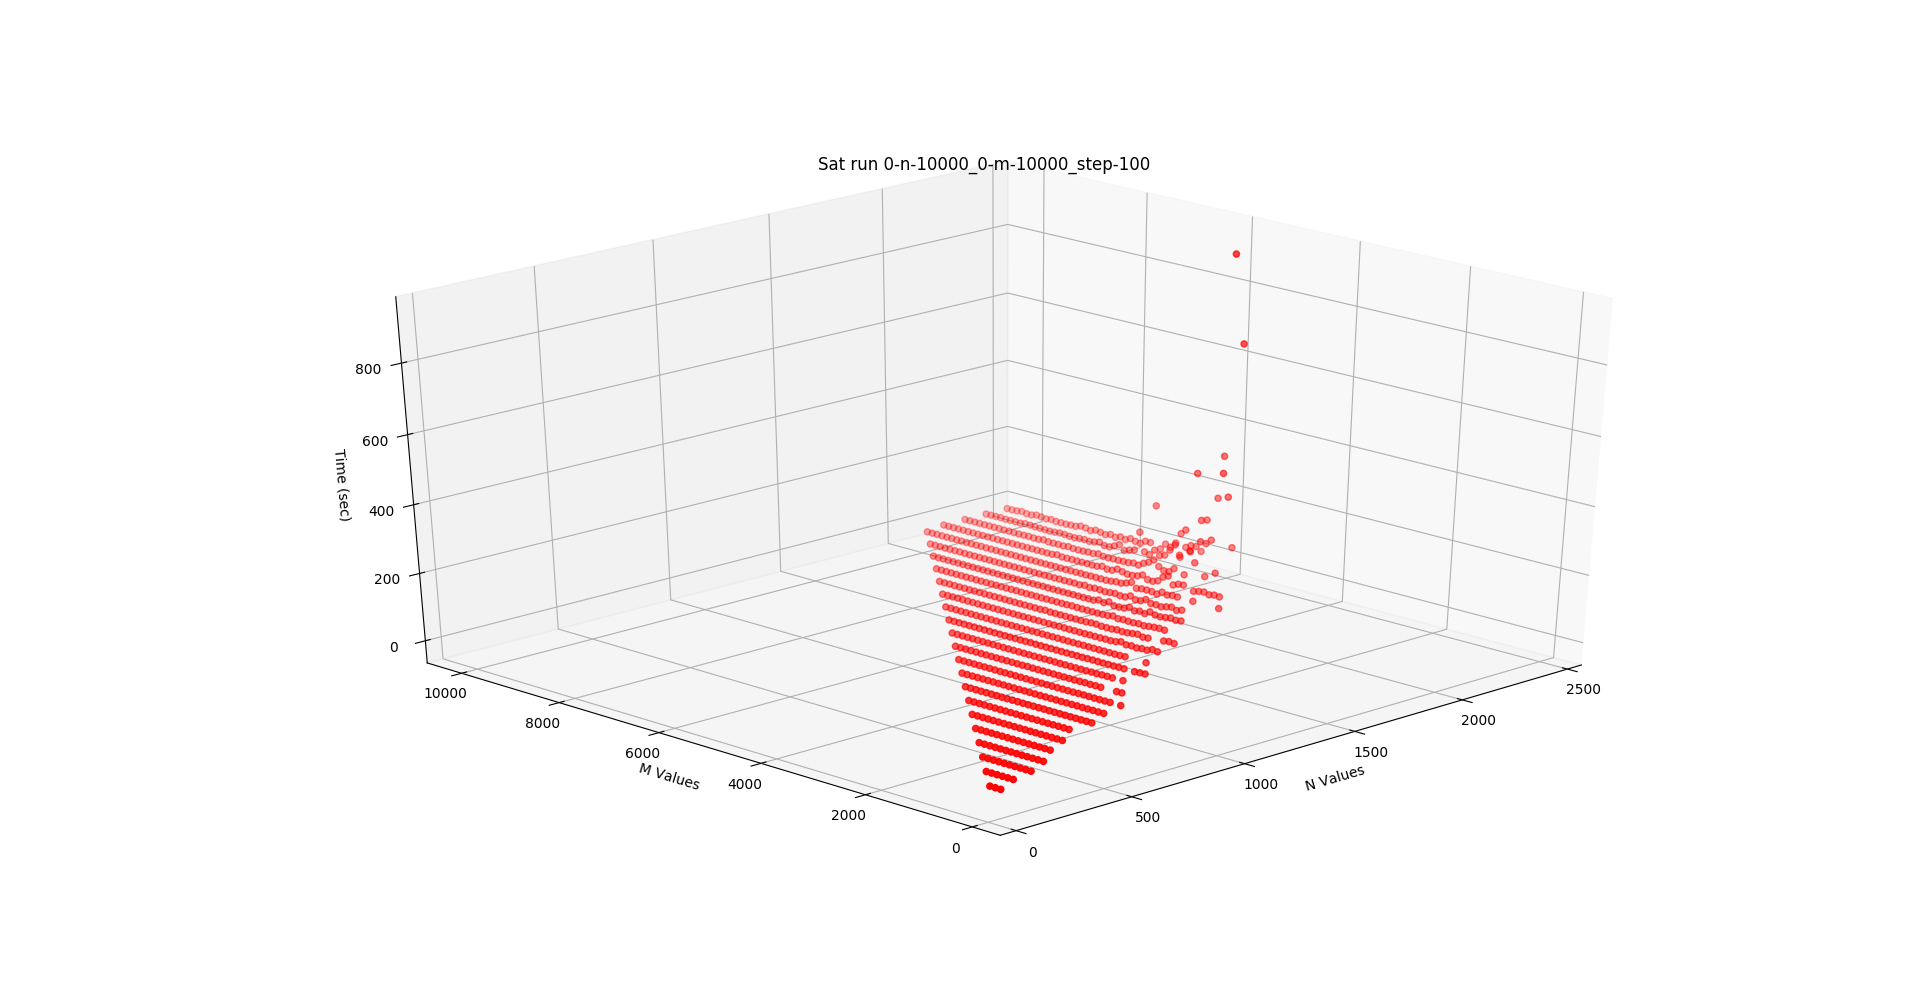
\includegraphics[height=75mm]{Figs/system_search_time}
	\caption{Time taken to search for uniquely satisfiable instances}
	\label{fig:sa}
\end{figure}

(Note that many graphical representations have rendered values illegible. To this end, we will describe some verbally, but retain enlarged images in our package. Such results were not saved as values, but kept as images after long running experiments.)

The $x$ axis represents variables $n$, $y$ represents clauses $m$ and the $z$ axis represents time taken to locate in seconds. This figure was produced after recording the time taken to find a uniquely satisfiable system of equations for combinations of $n$ and $m$. Hence, what we mean by the $2n=m$ line, are those instances which satisfy that equation (e.g. $n=10$ and $m=20$). This is an important distinction ot make, as we see that instances along certain lines differ in time taken to find, namely, those that are rightmost, that is, close to the threshold of satisfiability $n=m$ (the left is bounded by $3n=m$). Figure \ref{fig:sa} shows the cumulative time taken to locate each instance, which means each point includes failures and regenerating and testing instances for unique satisfiability (not necessarily $k$-locally consistent). It does not describe the validation time by Cryptominisat for a single instance, but does hint at this. Figure \ref{fig:sb} illustrates that we have to try much harder near the line of satisfiability to generate uniquely satisfiable systems, shown by the increase in time to the right. We see that for a single instance to be located, it took more than a hour to find a suitable instances near the $n=2000$ and $m=6000$ mark. One point to make, is that the number of tries stays the same. The empty space above lines $n=m$ and below the rightmost plots are instances which were not located using 10 attempts. Hence, it is not only becomes more unlikely to find instances, it also becomes more timely to validate them.

\begin{figure}[htbp!] 
	\centering
	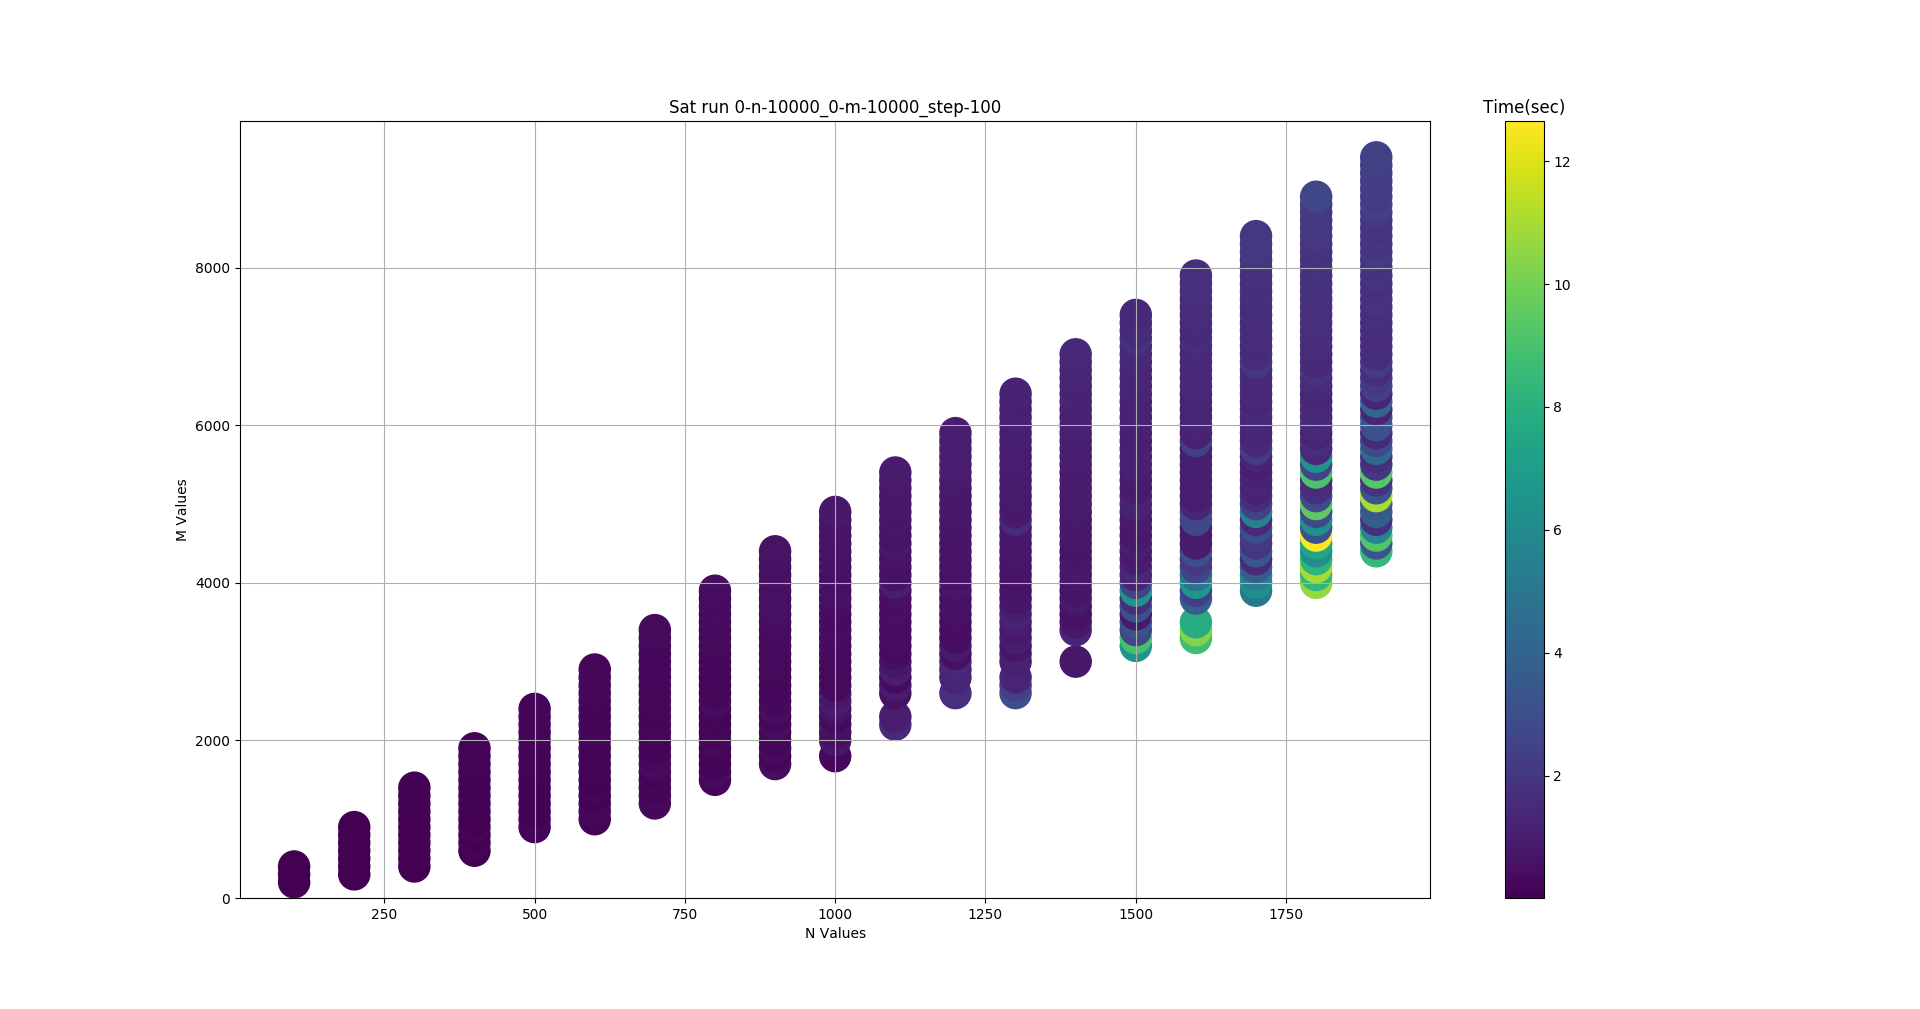
\includegraphics[height=75mm]{Figs/figure_1}
	\caption{Plot of various systems found.}{Note that instances close to the $n=m$ line take far greater time in validation.}
	\label{fig:sb}
\end{figure}

\newpage

\subsection{Validation}
Ensuring we had our desired constructions meant we had to make three checks: $k$-local consistency and unique satisfiability by Cryptominisat, and automorphisms on our preliminary graph using Traces. (Checking for automorphisms is left to Section \ref{sec:aut}.) 

\subsubsection{Unique satisfiability}
Aforementioned, the time taken to check for unique satisfiability increases along the threshold of satisfiability with respect to the size of the systems. Figure \ref{fig:hm} shows this.

\begin{figure}[htbp!] 
	\centering
	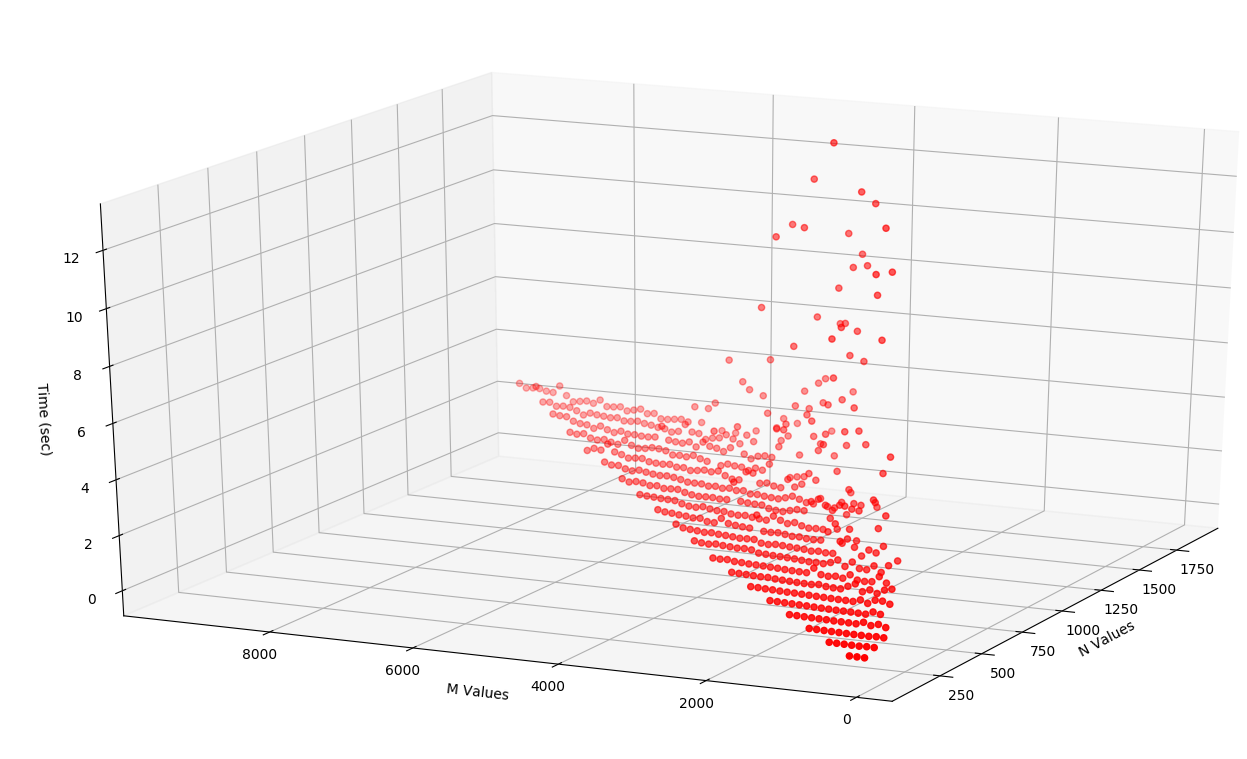
\includegraphics[height=75mm]{Figs/figure_2}
	\caption{Time taken to validate unique satisfiability using Gauss Off}
	\label{fig:hm}
\end{figure}

We note that Cryptominisat works faster with Gauss-Off feature versus Gauss-On. This is Counter-intuitive, since XOR-SAT is known to have a P-Time algorithm using Gaussian elimination. Evidently, validation of unique satisfiability systems, which are along the threshold, appear to take a vastly greater time than those further away. 

\newpage

\subsubsection{$k$-local consistency}
Our makeshift $k$-local consistency check found systems which were significantly quicker using Gauss-On versus Gauss-Off. In our Advanced Search, where we updated our store of slow running systems, that is, with the greatest difference in Gauss-On and Gauss-Off times. The following figure shows systems with negative plots are pseudo k-locally consistent. See Figure \ref{fig:kloc} below.

\begin{figure}[htbp!] 
	\centering
	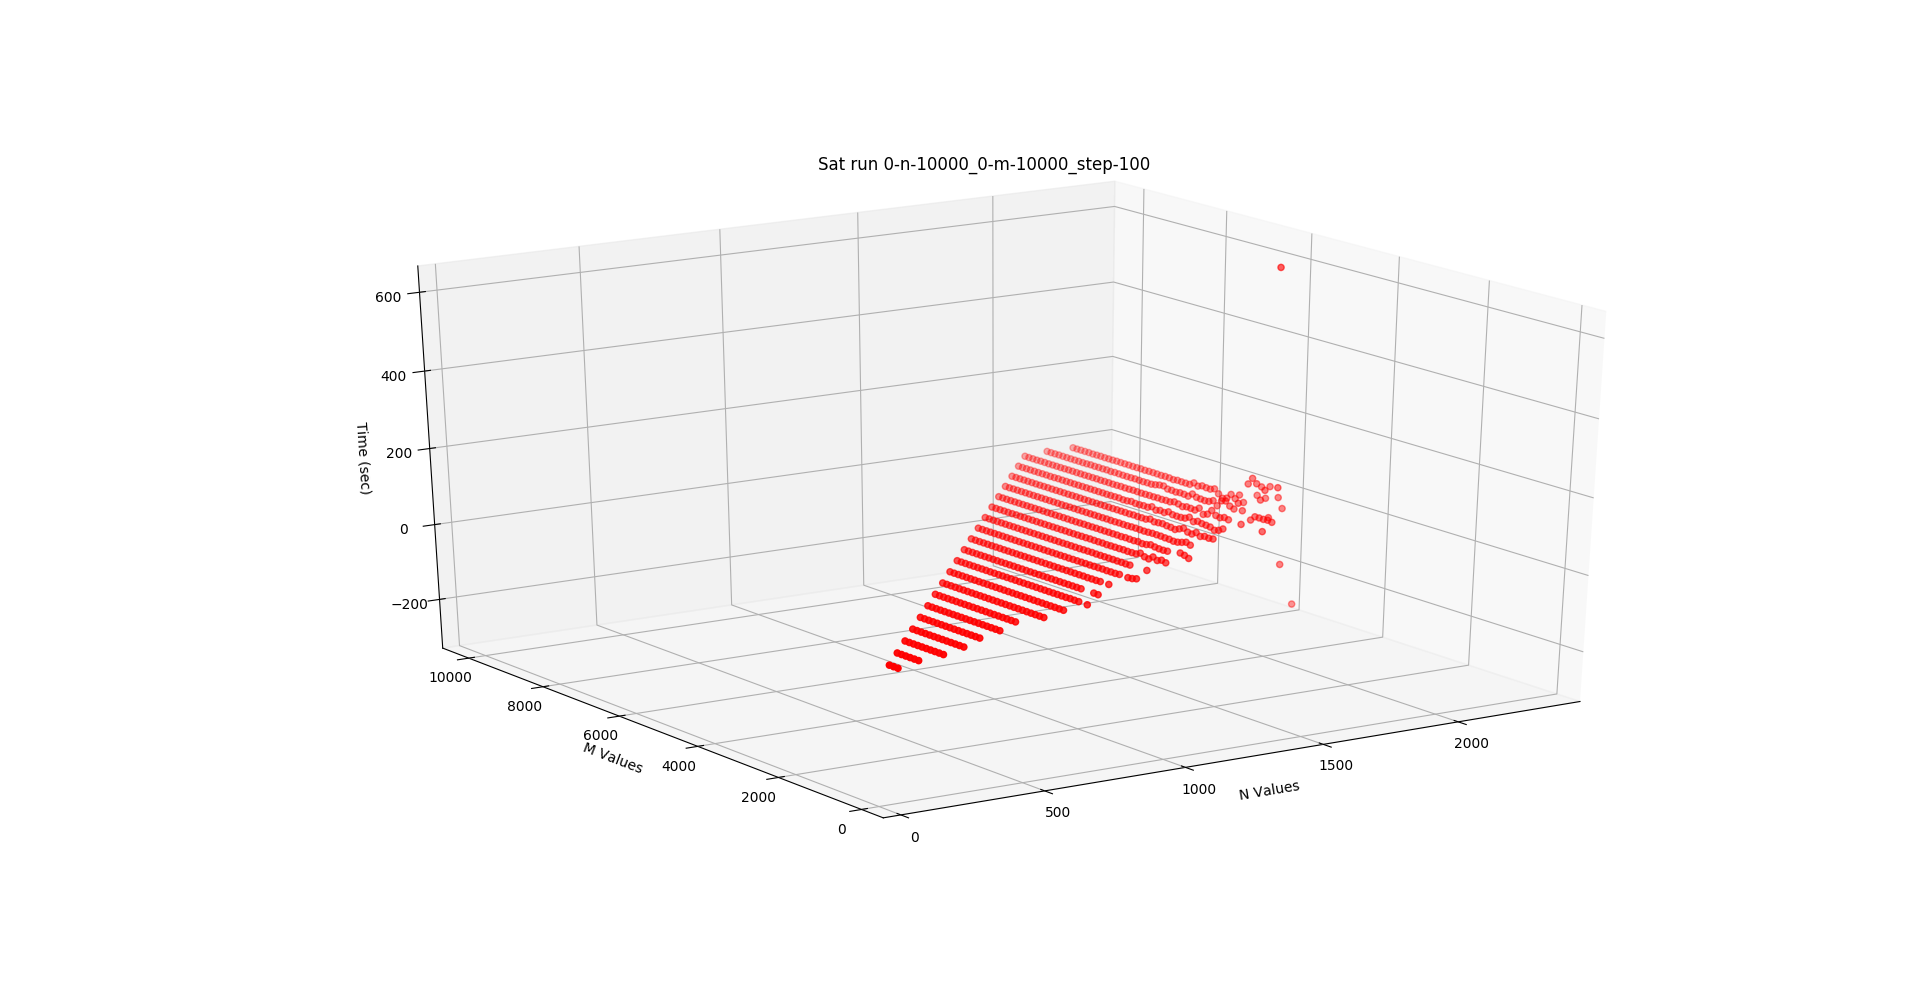
\includegraphics[height=75mm]{Figs/diff_3d}
	\caption{Time taken to validate unique satisfiability Gauss On - Gauss Off.}
	\label{fig:kloc}
\end{figure}

Notice that is more difficult to detect $k$-local consistency the further we move away from the threshold $n=m$. The difference in running times are fairly similar away from $n=m$, but erratic close to $n=m$. Especially as we increase the size of the systems. To which the boundary also moves further away from the line. 

\subsubsection{Strengthening}
As we will prove later, the larger difference between a Gauss-On and Gauss-Off execution time, where Gauss-On is faster for a given uniquely satisfiable 3-XOR-Formula $\phi$, the slower the final graph $G_B$ will be after transforming $\phi$ to $G_B$. Recall that in our Advanced Search we provide the facility to save the slowest found $\phi$. By repeating system searches, and continuously updating the slowest found $\phi$, we filter out very slow systems from the pool of random uniquely satisfiable systems. Hence, repeating a system search 30 times for specific instances, say $n=100$ and $m=100$, we can hope to find a strong instance which is slow for that value of $n$ and $m$. However, it is critical to note that for these values, systems must be readily available and not scarce. 

\newpage

\subsection{Varying Tries}
As we search for instances close to the line of satisfiability $n=m$, our desired construction becomes much more difficult to locate. Recall that the tries parameter in our systems search determines how many times to generate $\phi$ before quitting. 

We noticed that as $n$ and $m$ became larger, if we fixed the number of tries, then it would become more difficult to find instances close to the line of satisfiability. That is to say, as $n$ and $m$ increased, there would be a point where finding $2n=m$ would require more random generations to produce a desired instance, similarly with $3n=m$ and so on. This is better illustrated, but not accurately shown, in Figure \ref{fig:dif} below. The figure depicts that as values of $n$ and $m$ increase, instances along certain lines become scarce. This is important to note, since if we scarcely find instances at certain points, requiring a greater number of tries to locate, we are less likely to filter out a $k$-locally consistent system through repeating runs.

One notable test that can be reproduced is searching along $n=m$, and setting the number of attempts to a large 100,000 attempts to generate a system. One would find that desired instances are hardly available above the $n=m=100$ mark. We know such instances exist, but it becomes increasingly difficult to find an instance for say $n=m=150$. The largest $\phi$ we found for this ratio of $n$ and $m$ is 139, but this was not necessarily $k$-locally consistent as we generated this in 1 run: this is due to scarcely seeing graphs between 105 and 139, that is, many instances exceeded the 100,000 try value. Those below 100 were easy to find (10 tries), and strong systems were found after many iterations, but the same cannot be said for $n>105$, although, this would be ideal since it would produce slow running graphs.

\begin{figure}[h]
	\centering
	\begin{tikzpicture}[trim left=0cm, scale=0.8]
	\begin{axis}[
		xlabel={$n$},
		ylabel=Tries required to locate,
		grid=both,
		extra tick style={grid=major, grid style={dotted, cyan}},
		extra y tick labels={\hspace{5em}$timeout$},
		extra x tick labels={},
		extra y tick style={grid=none},
		yticklabels={,,},
		xticklabels={,,},
		axis lines = left,
		xmin=0,
		clip right=false,
		ymin=0,
		legend pos = north west,
	]
	\addplot[green]  {pow(2,x)};
	\addplot[black]  {pow(2,x-1)};
	\addplot[red]  {pow(2,x-2)};
	\addlegendentry{$n=m$};
	\addlegendentry{$2n=m$};
	\addlegendentry{$3n=m$};
	\end{axis}
	\end{tikzpicture}
	\caption{Illustration of instances becoming scarce}
	\label{fig:dif}
\end{figure}

\newpage
\subsection{Varying Step Size}
In our packages we provide systems and graphs which increase in size by some step factor, as defined in Table \ref{tab:parm}. If we vary the number of steps, we alter the amount of systems produces by our systems search, and ultimately how many graphs are generated. For some packages, for example $con\_n$, we have a step size of 1 between $6<n<10$, which increases to 10 at $10<n<100$, but then decreases to 1 between $100<n<150$. Recall that as instances become larger, they are begin to be scarcely available, which is prominent in the $n=m$ case. 

\subsection{Bounds}
In searching and constructing our graphs, we hit multiple bounds on what we could find. Such bounds are purely time constraints. For example, we decided to stop searching systems above $n=3000$, since our final graph $G_B$ would undoubtedly take longer than three hours to determine $Aut(G)$. A graph of $n=3000$ would result in $G_B$ having at least $18,000$ nodes. Figure \ref{fig:py} shows it was not necessary to generate graphs at this scale. Nonetheless, uniquely satisfiable instances were found at this range. Moreover, the time taken to validate such a system became large; Figure \ref{fig:sa} shows that it would take longer than 800s to find and validate such systems. We do not supplement uniquely satisfiable systems above $n=2500$ and do not provide graphs above $n=1000$ for these reasons.

\subsection{Timings}
Given that our construction is a graph which we test for automorphism that corresponds to a uniquely satisfiable and $k$-locally consistent 3-XOR-Formula, and that such a construction is tested on two types of solver, we provide a table of figures to see the overall performance. It should be emphasised that these times are based on the time taken to execute system calls initiated by Python, rather than actual CPU time for processes. Since Cryptominisat does not have such an inbuilt feature to show these values, we provide a subset of times for Traces $Aut(G_B)$ and Cryptominisat $uniquely\_satisfiable(\phi)$ using Gauss-Off. To save space, we refer to Appendix \ref{tim}. In total, Table \ref{table:pix} tells us the percentage of instances which timed out in our provided packages.

\begin{table}[htbp!]
	\centering
	\begin{tabular}{|c|c|c|c|}
	\hline
	Package & Largest Graph $n:m$ & Graphs & \% of Timeouts\\ \hline
	con\_sml & 1000:1700 & 95 & 21\% \\
	con\_n & 139:139 & 35 &  0\% \\ 
	con\_2n & 1000:2000 & 59 & 22\% \\ \hline
	\end{tabular}
	\caption{Percentage of graphs which took longer than three hours to execute on Traces}
	\label{table:pix}
	
\end{table}

\newpage

\section{Preliminary Graph Automorphism Test}\label{sec:aut}
Since we want our graphs with no non-trivial automorphisms, we must validate that a given system when translated into our preliminary representation has this attribute. See Figure \ref{fig:avb}

We found that testing graph $G_A$ was a fairly fast check, and executed at most after a few seconds. This led to the integration of this check into our advanced search as a feature. The following figure shows run times of some preliminary graphs for automorphisms versus the corresponding final construction. We see the significance and drastic increase in execution times once we apply the multipede transformation.  

\begin{figure}[h] 
	\centering
	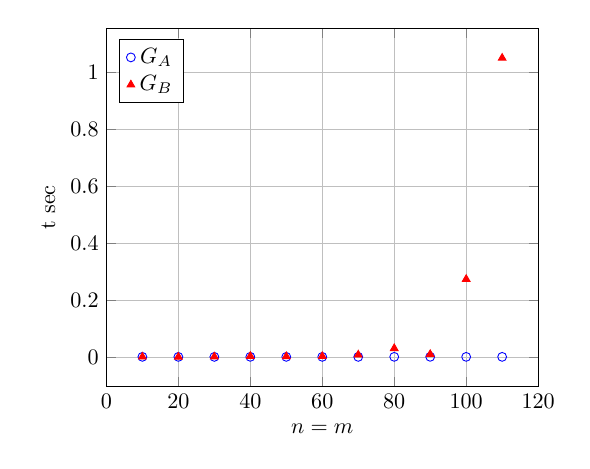
\begin{tikzpicture}[trim left=-1cm, scale=0.8]
	\begin{axis}[
	xlabel={$n=m$},
	ylabel=t sec,
	grid=both,
	legend pos=north west,
	extra tick style={grid=major, grid style={dotted, cyan}},
	extra x tick labels={},
	extra y tick style={grid=none}
	]
	\addplot[
	scatter,only marks,scatter src=explicit symbolic,
	scatter/classes={
		a={mark=o,blue},
		b={mark=triangle*,red}
	}
	]
	table[x=x,y=y,meta=label]{
		x    y    label
		10  0.000648975372314 a
		10  0.000707864761353 b
		20  0.000533103942871 a
		20  0.000607013702393 b
		30  0.000514030456543 a
		30  0.00131988525391 b
		40  0.000682830810547 a
		40  0.00321912765503 b
		50  0.000607013702393 a
		50  0.00205492973328 b
		60  0.000588893890381 a
		60  0.00267696380615 b
		70  0.000577926635742 a
		70  0.00788307189941 b
		80  0.000648975372314 a
		80  0.0305290222168 b
		90  0.000776052474976 a
		90  0.00965595245361 b
		100  0.000566959381104 a
		100  0.273800849915 b
		110  0.000571012496948 a
		110  1.05121898651 b
	};
	\legend{$G_A$, $G_B$}
	\end{axis}
	\end{tikzpicture}
	\caption{Graph $G_A$ versus $G_B$ for $n=m$}
	\label{fig:avb}
\end{figure}

\section{k-local Consistency Experimental Proof}
Here we provide experimental proof that using gauss elimination on versus off did indeed make a difference in times. We take graphs of two identical sizes, $n=300$ and $m=600$. For one system, we generated a uniquely satisfiable set of clauses without checking our stored version, which is the other. We convert both systems into graphs and find that one system is substantially slower than the other. We see that a system with a large  discrepancy in time gives rise to a drastically slower system. See Table \ref{table:tx}.

\begin{table}[h]
	\centering
	\begin{tabular}{l l l l}
		\toprule
		Instance 300:600 ($n:m$)& Gauss On & Gauss Off & Traces time  \\ 
		\midrule
		Random uniquely satisfiable system & 0.0078 & 0.0077 & 0.18 \\
		Likely $k$-locally consistent & 0.0074 & 0.0129 & 1.04 \\
		\bottomrule
	\end{tabular}
	\caption{Comparing two graphs. Both are $2n=m$ with $n=300$ and $m=600$}
	\label{table:tx}
	
\end{table}



